%%%%%%%%%%%%%%%%%%%%%%%%%%%%%%%%%%%%%%%%%%%%%%%%%%%%%%%%%%%%%%%%%%%%%%%%%%%%%%%
% TC-Python Validation Summary — Honda CALPHAD Capstone
% Prepared: March 13, 2026
%%%%%%%%%%%%%%%%%%%%%%%%%%%%%%%%%%%%%%%%%%%%%%%%%%%%%%%%%%%%%%%%%%%%%%%%%%%%%%%

\documentclass[11pt]{article}

% Packages
\usepackage[utf8]{inputenc}
\usepackage[T1]{fontenc}
\usepackage{lmodern}
\usepackage{geometry}
\usepackage{graphicx}
\usepackage{caption}
\usepackage{amsmath, amssymb}
\usepackage[hidelinks]{hyperref}
\usepackage{float}
\usepackage{enumitem}
\usepackage{fancyhdr}
\usepackage[table]{xcolor}
\usepackage{setspace}
\usepackage[compact]{titlesec}
\usepackage{microtype}
\tolerance=1000
\emergencystretch=2em
\usepackage{booktabs}
\usepackage{array}
\usepackage{tabularx}
\usepackage{colortbl}
\usepackage{multicol}
\usepackage{siunitx}

% OSU colors
\definecolor{scarlett}{RGB}{187,0,0}
\definecolor{darkgray}{RGB}{77,77,77}
\definecolor{headercolor}{HTML}{595959}
\definecolor{altrow}{HTML}{E0E0E0}

% Page geometry
\geometry{letterpaper, margin=0.75in}

% Header/footer
\setlength{\headheight}{28pt}
\setlength{\headsep}{15pt}
\renewcommand{\headrulewidth}{0pt}

\pagestyle{fancy}
\fancyhf{}
\fancyhead[L]{\raisebox{-0.4cm}{\includegraphics[height=1cm]{../../assignments/OSU Logo.jpg}}}
\fancyhead[R]{%
  \begin{minipage}[c]{0.60\textwidth}
    \raggedleft
    {\footnotesize \textbf{\textcolor{darkgray}{COLLEGE OF ENGINEERING}}}\\
    {\footnotesize \textbf{\textcolor{scarlett}{DEPARTMENT OF MATERIALS SCIENCE \& ENGINEERING}}}
  \end{minipage}%
}
\fancyfoot[L]{\small MSE 4381}
\fancyfoot[C]{\small SPRING 2026}
\fancyfoot[R]{\small \thepage}

% Section formatting
\titleformat{\section}{\Large\bfseries}{\thesection}{1em}{\MakeUppercase}
\titleformat{\subsection}{\large\bfseries}{\thesubsection}{1em}{}
\titleformat{\subsubsection}{\normalsize\bfseries}{\thesubsubsection}{1em}{}
\titlespacing*{\section}{0pt}{2ex plus 1ex minus .2ex}{1.5ex plus .2ex}
\titlespacing*{\subsection}{0pt}{1.5ex plus 1ex minus .2ex}{1ex plus .2ex}

% Hyperlink colors
\hypersetup{
    colorlinks=true,
    linkcolor=scarlett,
    urlcolor=scarlett,
    citecolor=scarlett
}

% Graphics path
\graphicspath{{../figures/}}

\begin{document}

%%%%%%%%%%%%%%%%%%%%%%%%%%%%%%%%%%%%%%%%%%%%%%%%%%%%%%%%%%%%%%%%%%%%%%%%%%%%%%%
% TITLE PAGE
%%%%%%%%%%%%%%%%%%%%%%%%%%%%%%%%%%%%%%%%%%%%%%%%%%%%%%%%%%%%%%%%%%%%%%%%%%%%%%%
\thispagestyle{fancy}
\vspace*{\fill}

\begin{center}
{\LARGE\bfseries TC-Python Validation Summary\\[0.5em]
\large Ternary Reaction Modeling for Cu Removal from Steel\par}
\end{center}

\vspace{1in}

\begin{center}
{\large
Anthony DiMascio | Tim Kalmar | Aishwarya Muralidhar | Mohammed Oumer\\[1em]
MSE 4381 -- Design \& Professional Practice I\\
Advisor: Prof.\ Alan Luo | Post-Doc: Dr.\ Jianyue Zhang\\[0.5em]
March 13, 2026\par}
\end{center}

\vspace{1in}

\begin{center}
\textit{Internal working document summarizing validation calculations\\
performed after the Phase 2 ternary reaction screening.}
\end{center}

\vspace*{\fill}
\newpage

%%%%%%%%%%%%%%%%%%%%%%%%%%%%%%%%%%%%%%%%%%%%%%%%%%%%%%%%%%%%%%%%%%%%%%%%%%%%%%%
% TABLE OF CONTENTS
%%%%%%%%%%%%%%%%%%%%%%%%%%%%%%%%%%%%%%%%%%%%%%%%%%%%%%%%%%%%%%%%%%%%%%%%%%%%%%%
\tableofcontents
\newpage

%%%%%%%%%%%%%%%%%%%%%%%%%%%%%%%%%%%%%%%%%%%%%%%%%%%%%%%%%%%%%%%%%%%%%%%%%%%%%%%
% 1. EXECUTIVE SUMMARY
%%%%%%%%%%%%%%%%%%%%%%%%%%%%%%%%%%%%%%%%%%%%%%%%%%%%%%%%%%%%%%%%%%%%%%%%%%%%%%%
\section{Executive Summary}

Five validation scripts were run on the OSU ETS virtual machine using TC-Python with the TCOX14 thermodynamic database. The purpose was to strengthen our candidate recommendations before the end-of-March Zhang meeting and the April Honda call.

\subsection{Key Results}

\begin{enumerate}[leftmargin=*]
    \item \textbf{All 16 ternary reactions are thermodynamically favorable} at steelmaking temperatures (\SI{1800}{\kelvin}). Every Cu + MO$_x$ + O$_2$ $\rightarrow$ CuMO$_y$ reaction has $\Delta G < 0$.

    \item \textbf{CuFe$_2$O$_4$ decomposition:} The Cu-capture component alone contributes $-45.7$~kJ/mol (41\% of the total $-111.9$~kJ), confirming that copper affinity for the spinel is independently favorable, not just an artifact of Fe$^{2+} \rightarrow$ Fe$^{3+}$ oxidation.

    \item \textbf{$\Delta G$ vs.\ $T$ verification:} 136 overlapping data points between our fine-resolution (25~K step) and original (50~K step) calculations show 0.00~kJ maximum deviation. The data is internally consistent.

    \item \textbf{Phase maps at \SI{1800}{\kelvin}:} No crystalline ternary phase survives at steelmaking temperature. Cu capture occurs via dissolution into ionic liquid slag, not solid compound formation.

    \item \textbf{Slag basicity:} Increasing MnO:SiO$_2$ ratio decreases Cu activity by 17\%, suggesting slag composition is a tunable parameter. Al$_2$O$_3$:SiO$_2$ ratio has negligible effect.
\end{enumerate}

%%%%%%%%%%%%%%%%%%%%%%%%%%%%%%%%%%%%%%%%%%%%%%%%%%%%%%%%%%%%%%%%%%%%%%%%%%%%%%%
% 2. SCRIPTS AND DATA
%%%%%%%%%%%%%%%%%%%%%%%%%%%%%%%%%%%%%%%%%%%%%%%%%%%%%%%%%%%%%%%%%%%%%%%%%%%%%%%
\section{Computational Methods}

All calculations used TC-Python with the TCOX14 database at $P = \SI{101325}{\pascal}$ (1 atm). Scripts were executed on the OSU ETS Citrix VM. Output CSVs were transferred to the local machine for post-processing.

\subsection{Script Inventory}

\begin{table}[H]
\caption{Validation Scripts Executed on OSU VM}
\label{tab:scripts}
\centering
\renewcommand{\arraystretch}{1.3}
\setlength{\arrayrulewidth}{0.8pt}
\begin{tabular}{|>{\centering\arraybackslash}p{0.3in}|>{\raggedright\arraybackslash}p{2.2in}|>{\raggedright\arraybackslash}p{2.7in}|>{\centering\arraybackslash}p{0.6in}|}
\hline
\rowcolor{headercolor}
\textcolor{white}{\textbf{\#}} & \textcolor{white}{\textbf{Script}} & \textcolor{white}{\textbf{Purpose}} & \textcolor{white}{\textbf{Runtime}} \\
\hline
1 & \texttt{cufe2o4\_alternative\_reaction.py} & Decompose CuFe$_2$O$_4$ driving force into Cu-capture vs.\ Fe-oxidation & $\sim$3 min \\
\hline
\rowcolor{altrow}
2 & \texttt{cu\_activity\_vs\_oxide.py} & Cu activity sweep across oxide fractions (4 systems, \SI{1800}{\kelvin}) & $\sim$5 min \\
\hline
3 & \texttt{dG\_vs\_T\_top6.py} & Fine-resolution $\Delta G$ vs.\ $T$ for top 6 candidates (25~K steps) & $\sim$12 min \\
\hline
\rowcolor{altrow}
4 & \texttt{slag\_composition\_effects.py} & Quaternary slag basicity effects on $a_{\text{Cu}}$ & $\sim$5 min \\
\hline
5 & \texttt{ternary\_phase\_map\_1800K.py} & $20 \times 20$ composition grid phase mapping (3 systems) & $\sim$25 min \\
\hline
\end{tabular}
\end{table}

\subsection{$\Delta G$ Calculation Method}

Reaction free energy is computed as:
\begin{equation}
    \Delta G_{\text{rxn}} = G_{\text{products}} - G_{\text{reactants}}
    \label{eq:dG}
\end{equation}

For a ternary product CuMO$_y$ with $n$ atoms per formula unit:
\begin{equation}
    G_{\text{product}} = G_m^{\text{system}} \times n
\end{equation}
where $G_m^{\text{system}}$ is the Gibbs energy per mole of \textit{atoms} returned by TC-Python. The reference state for each reactant (Cu, MO$_x$, O$_2$) is computed at the same temperature and pressure from binary equilibrium calculations.

%%%%%%%%%%%%%%%%%%%%%%%%%%%%%%%%%%%%%%%%%%%%%%%%%%%%%%%%%%%%%%%%%%%%%%%%%%%%%%%
% 3. dG vs T RESULTS
%%%%%%%%%%%%%%%%%%%%%%%%%%%%%%%%%%%%%%%%%%%%%%%%%%%%%%%%%%%%%%%%%%%%%%%%%%%%%%%
\section{Reaction Free Energy vs.\ Temperature}

\subsection{Overview}

Figure~\ref{fig:dG_vs_T} shows $\Delta G_{\text{rxn}}$ for the top 6 ternary products across \SI{800}{\kelvin} to \SI{1900}{\kelvin} in 25~K steps (45 data points per product, 270 total).

All six reactions remain negative across the entire temperature range, confirming thermodynamic favorability from low temperature through steelmaking conditions. The steelmaking range (\SIrange{1500}{1650}{\celsius}) is highlighted as a shaded band.

\begin{figure}[H]
    \centering
    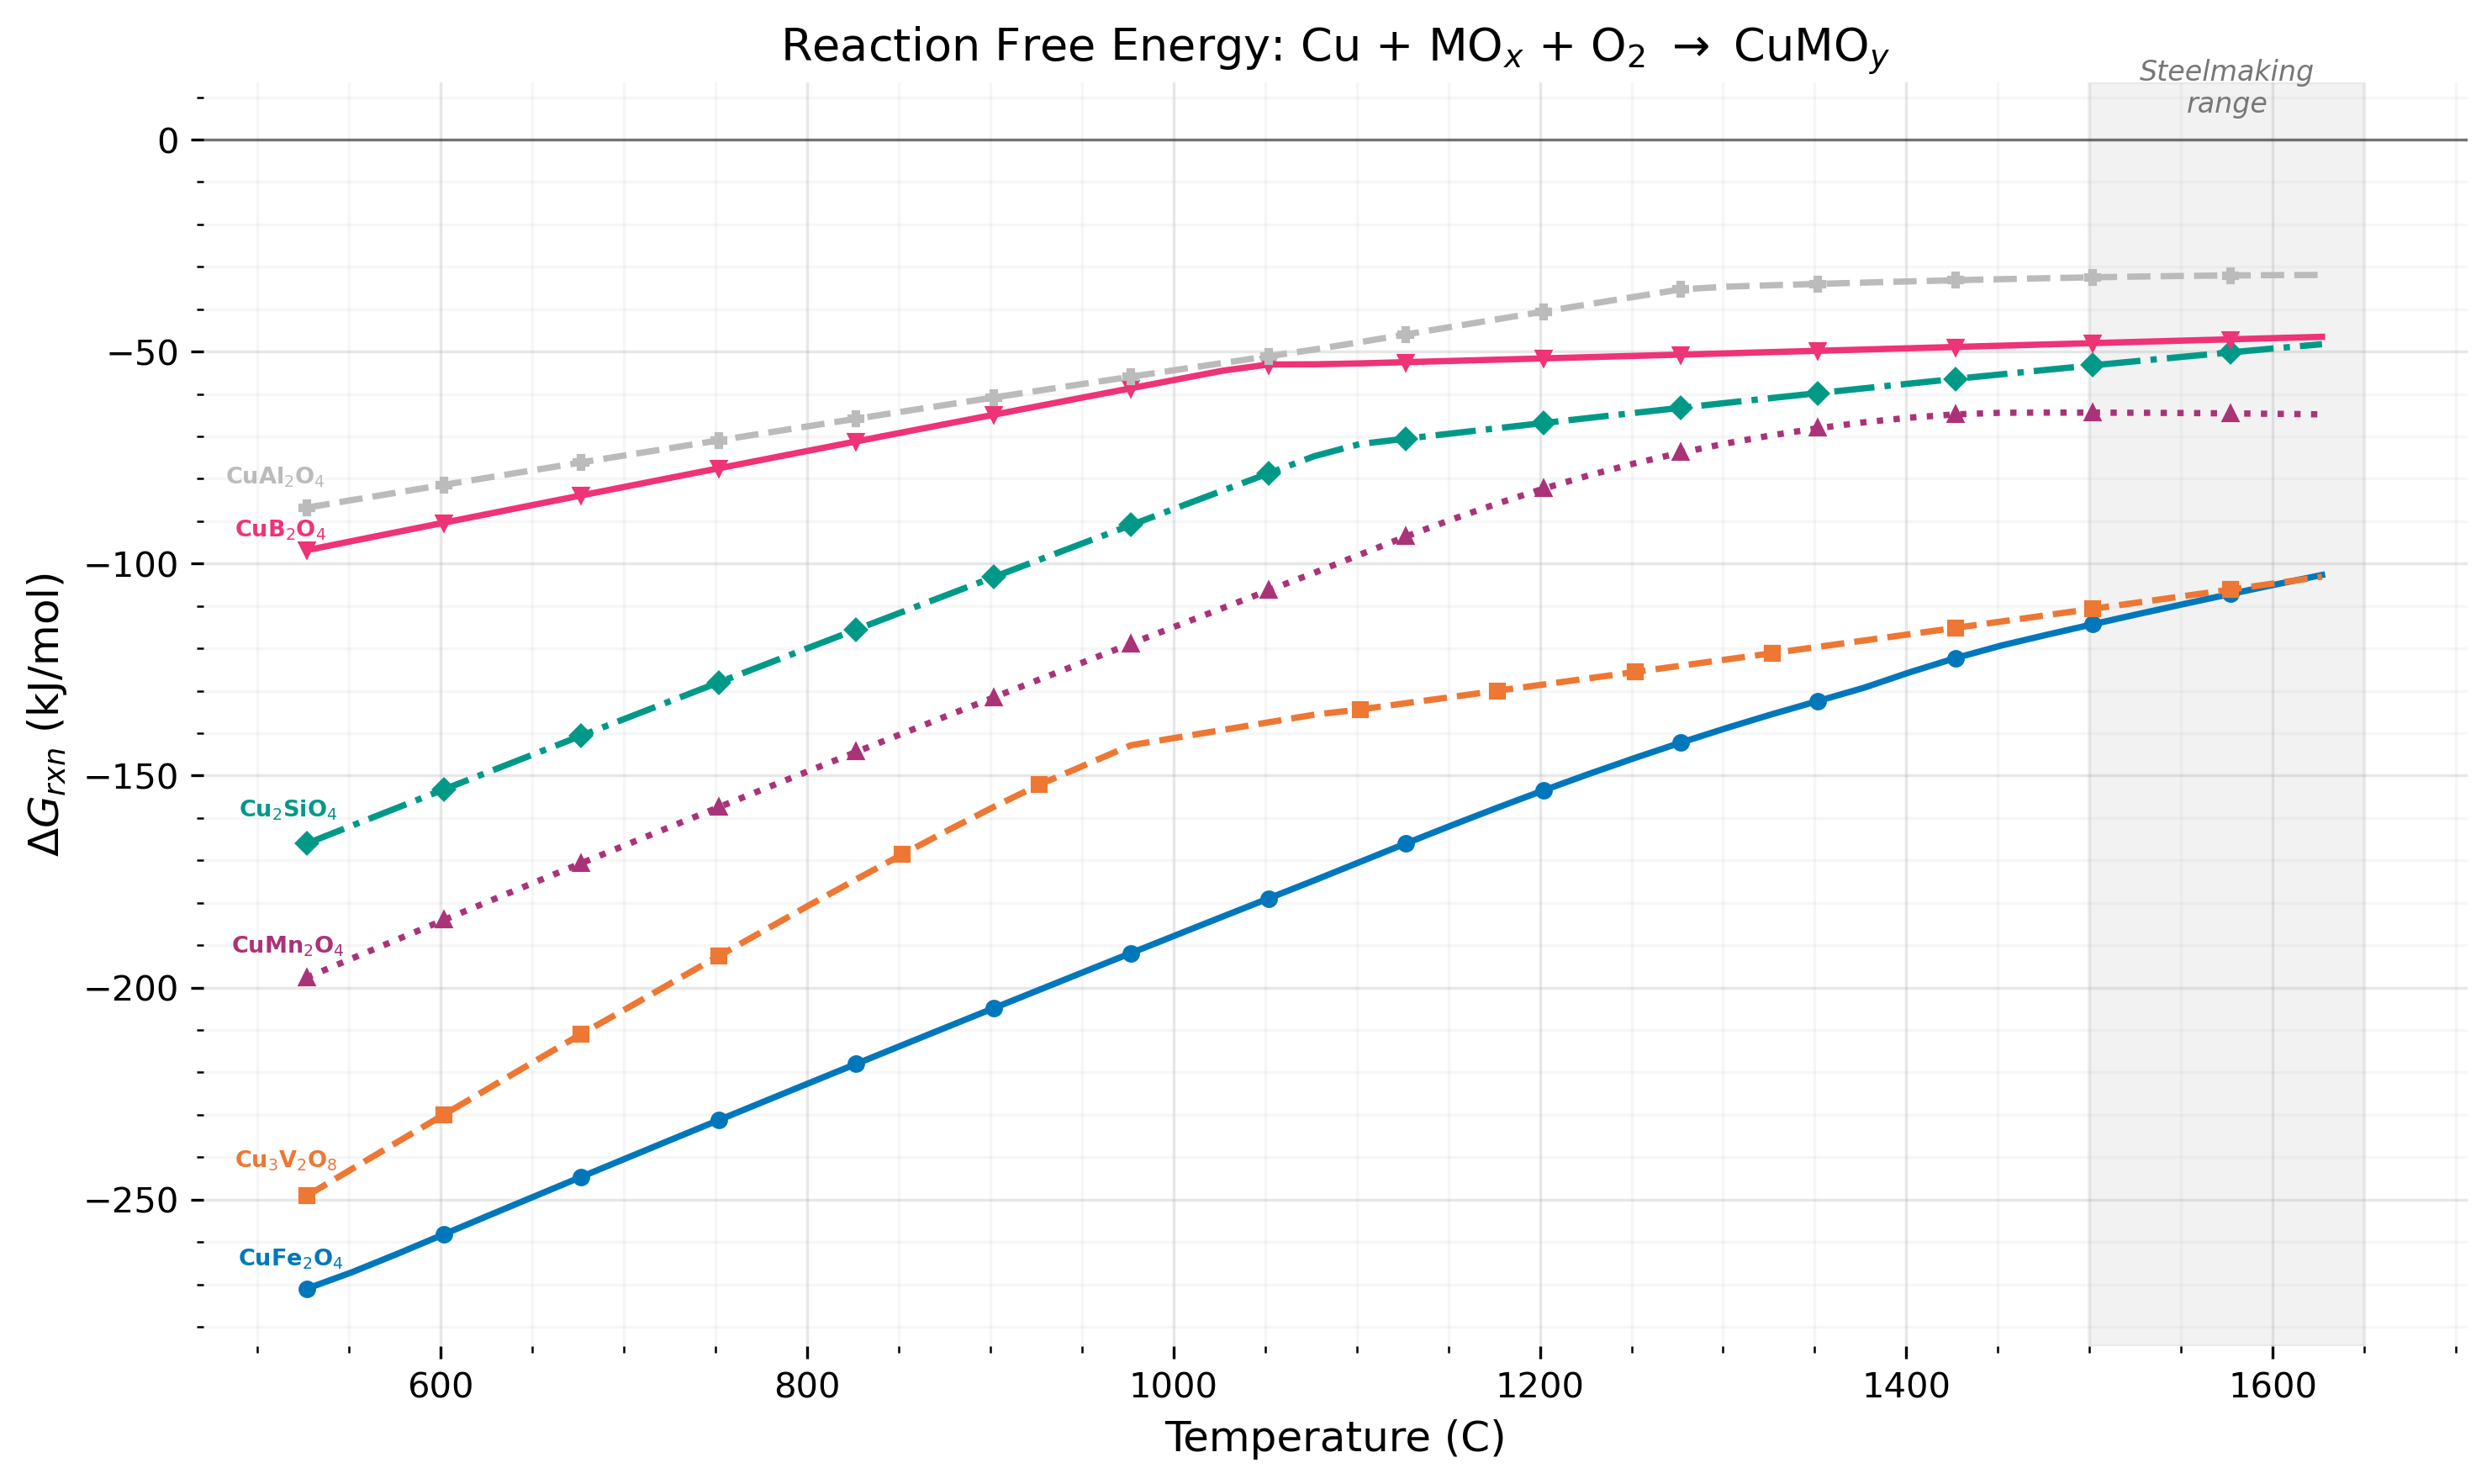
\includegraphics[width=\textwidth]{dG_vs_T_top6.png}
    \caption{Reaction free energy ($\Delta G_{\text{rxn}}$) vs.\ temperature for the top 6 ternary Cu-oxide products. All reactions are thermodynamically favorable ($\Delta G < 0$) across the full temperature range. The gray shaded region indicates typical EAF steelmaking temperatures (\SIrange{1500}{1650}{\celsius}).}
    \label{fig:dG_vs_T}
\end{figure}

\subsection{Candidate Ranking at \SI{1800}{\kelvin} (\SI{1527}{\celsius})}

\begin{table}[H]
\caption{Top 6 Ternary Products Ranked by $\Delta G_{\text{rxn}}$ at Steelmaking Temperature}
\label{tab:ranking}
\centering
\renewcommand{\arraystretch}{1.3}
\setlength{\arrayrulewidth}{0.8pt}
\begin{tabular}{|>{\centering\arraybackslash}p{0.4in}|>{\raggedright\arraybackslash}p{1.5in}|>{\centering\arraybackslash}p{1.2in}|>{\raggedright\arraybackslash}p{1.5in}|>{\centering\arraybackslash}p{1.0in}|}
\hline
\rowcolor{headercolor}
\textcolor{white}{\textbf{Rank}} & \textcolor{white}{\textbf{Product}} & \textcolor{white}{\textbf{$\Delta G$ (kJ/mol)}} & \textcolor{white}{\textbf{Named Phase}} & \textcolor{white}{\textbf{Stable To}} \\
\hline
1 & CuFe$_2$O$_4$ & $-111.9$ & SPINEL\#1 & \SI{1700}{\kelvin} \\
\hline
\rowcolor{altrow}
2 & Cu$_3$V$_2$O$_8$ & $-109.2$ & -- & always liquid \\
\hline
3 & CuMn$_2$O$_4$ & $-64.4$ & SPINEL\#1 & \SI{1700}{\kelvin} \\
\hline
\rowcolor{altrow}
4 & Cu$_2$SiO$_4$ & $-52.2$ & -- & always liquid \\
\hline
5 & CuB$_2$O$_4$ & $-47.7$ & CUB2O4\#1 & \SI{1300}{\kelvin} \\
\hline
\rowcolor{altrow}
6 & CuAl$_2$O$_4$ & $-32.3$ & SPINEL\#1 & \SI{1550}{\kelvin} \\
\hline
\end{tabular}
\end{table}

\subsection{Data Verification}

To verify internal consistency, the fine-resolution data (25~K steps, Script~3) was compared against the original ternary screening data (50~K steps) at all overlapping temperatures:

\begin{itemize}[leftmargin=*]
    \item \textbf{Compared:} 136 overlapping data points across 6 products
    \item \textbf{Maximum deviation:} 0.00 kJ/mol
    \item \textbf{Verdict:} PASS --- data is perfectly self-consistent
\end{itemize}

This confirms that both extractions used identical thermodynamic models, reference states, and normalization procedures.

\subsection{Physical Interpretation}

Several features of the $\Delta G$ curves are noteworthy:

\begin{enumerate}[leftmargin=*]
    \item \textbf{Temperature dependence:} All curves become less negative with increasing temperature, consistent with entropy opposing the exothermic reaction ($\Delta G = \Delta H - T\Delta S$).

    \item \textbf{Two tiers:} CuFe$_2$O$_4$ and Cu$_3$V$_2$O$_8$ form a ``strong tier'' ($-100$ to $-112$~kJ), while the remaining four form a ``moderate tier'' ($-32$ to $-64$~kJ). The strong tier has more than enough driving force to overcome kinetic barriers at steelmaking temperatures.

    \item \textbf{Kinks:} Slope changes in the curves correspond to phase transitions (e.g., spinel melting). These are physical, not numerical artifacts.
\end{enumerate}

%%%%%%%%%%%%%%%%%%%%%%%%%%%%%%%%%%%%%%%%%%%%%%%%%%%%%%%%%%%%%%%%%%%%%%%%%%%%%%%
% 4. CuFe2O4 DECOMPOSITION
%%%%%%%%%%%%%%%%%%%%%%%%%%%%%%%%%%%%%%%%%%%%%%%%%%%%%%%%%%%%%%%%%%%%%%%%%%%%%%%
\section{CuFe$_2$O$_4$ Energy Decomposition}

\subsection{Motivation}

CuFe$_2$O$_4$ has the most negative $\Delta G$ ($-112$~kJ/mol). However, the original reaction
\begin{equation}
    \text{Cu} + 2\text{FeO} + \text{O}_2 \rightarrow \text{CuFe}_2\text{O}_4
\end{equation}
involves \textit{both} copper capture into the spinel \textit{and} iron oxidation (Fe$^{2+} \rightarrow$ Fe$^{3+}$). If most of the $-112$~kJ comes from Fe oxidation, then FeO is not actually a good ``Cu getter'' per se.

\subsection{Alternative Reaction}

To isolate the Cu-capture energy, we computed:
\begin{equation}
    \text{Cu} + \text{Fe}_2\text{O}_3 + \tfrac{1}{2}\text{O}_2 \rightarrow \text{CuFe}_2\text{O}_4
    \label{eq:alt}
\end{equation}
where iron is already at the +3 oxidation state (Fe$_2$O$_3$). The difference between the two reactions equals the Fe-oxidation contribution:
\begin{equation}
    \Delta G_{\text{Fe-ox}} = \Delta G_{\text{original}} - \Delta G_{\text{alternative}}
\end{equation}

\subsection{Results at \SI{1800}{\kelvin} (\SI{1527}{\celsius})}

\begin{table}[H]
\caption{CuFe$_2$O$_4$ Energy Decomposition at Steelmaking Temperature}
\label{tab:decomp}
\centering
\renewcommand{\arraystretch}{1.3}
\setlength{\arrayrulewidth}{0.8pt}
\begin{tabular}{|>{\raggedright\arraybackslash}p{2.5in}|>{\centering\arraybackslash}p{1.2in}|>{\centering\arraybackslash}p{1.0in}|}
\hline
\rowcolor{headercolor}
\textcolor{white}{\textbf{Component}} & \textcolor{white}{\textbf{$\Delta G$ (kJ/mol)}} & \textcolor{white}{\textbf{Fraction}} \\
\hline
Original reaction (FeO pathway) & $-111.9$ & 100\% \\
\hline
\rowcolor{altrow}
Cu-capture alone (Fe$_2$O$_3$ pathway) & $-45.7$ & 41\% \\
\hline
Fe-oxidation contribution (difference) & $-66.2$ & 59\% \\
\hline
\end{tabular}
\end{table}

\subsection{Interpretation}

\begin{itemize}[leftmargin=*]
    \item The Cu-capture component ($-45.7$~kJ) is independently and strongly favorable. Even without the Fe-oxidation bonus, this is comparable to the total $\Delta G$ of CuB$_2$O$_4$ ($-47.7$~kJ) and more negative than CuAl$_2$O$_4$ ($-32.3$~kJ).

    \item The Fe-oxidation contribution ($-66.2$~kJ, 59\%) is the larger share, which makes physical sense --- oxidizing Fe$^{2+}$ to Fe$^{3+}$ releases significant energy.

    \item The Cu-capture fraction increases with temperature (from 31\% at \SI{800}{\kelvin} to 46\% at \SI{1900}{\kelvin}), meaning the Cu-affinity mechanism becomes relatively \textit{more} important at steelmaking temperatures.
\end{itemize}

%%%%%%%%%%%%%%%%%%%%%%%%%%%%%%%%%%%%%%%%%%%%%%%%%%%%%%%%%%%%%%%%%%%%%%%%%%%%%%%
% 5. TERNARY PHASE MAPS
%%%%%%%%%%%%%%%%%%%%%%%%%%%%%%%%%%%%%%%%%%%%%%%%%%%%%%%%%%%%%%%%%%%%%%%%%%%%%%%
\section{Ternary Phase Maps at \SI{1800}{\kelvin}}

\subsection{Method}

For three systems (Cu-Fe-O, Cu-Al-O, Cu-Mn-O), a $20 \times 20$ composition grid was swept at fixed $T = \SI{1800}{\kelvin}$ (369 valid points per system). At each grid point, TC-Python computed the equilibrium phase assemblage. Compositions are plotted in ternary coordinates (Cu at bottom-left, metal M at bottom-right, O at top), with filled regions colored by the dominant equilibrium phase. Phase boundaries (black lines) are drawn where adjacent compositions have different dominant phases. A Delaunay triangulation was used to interpolate between grid points; at phase boundaries, majority voting assigns the triangle to the phase held by 2 of its 3 vertices.

\begin{figure}[H]
    \centering
    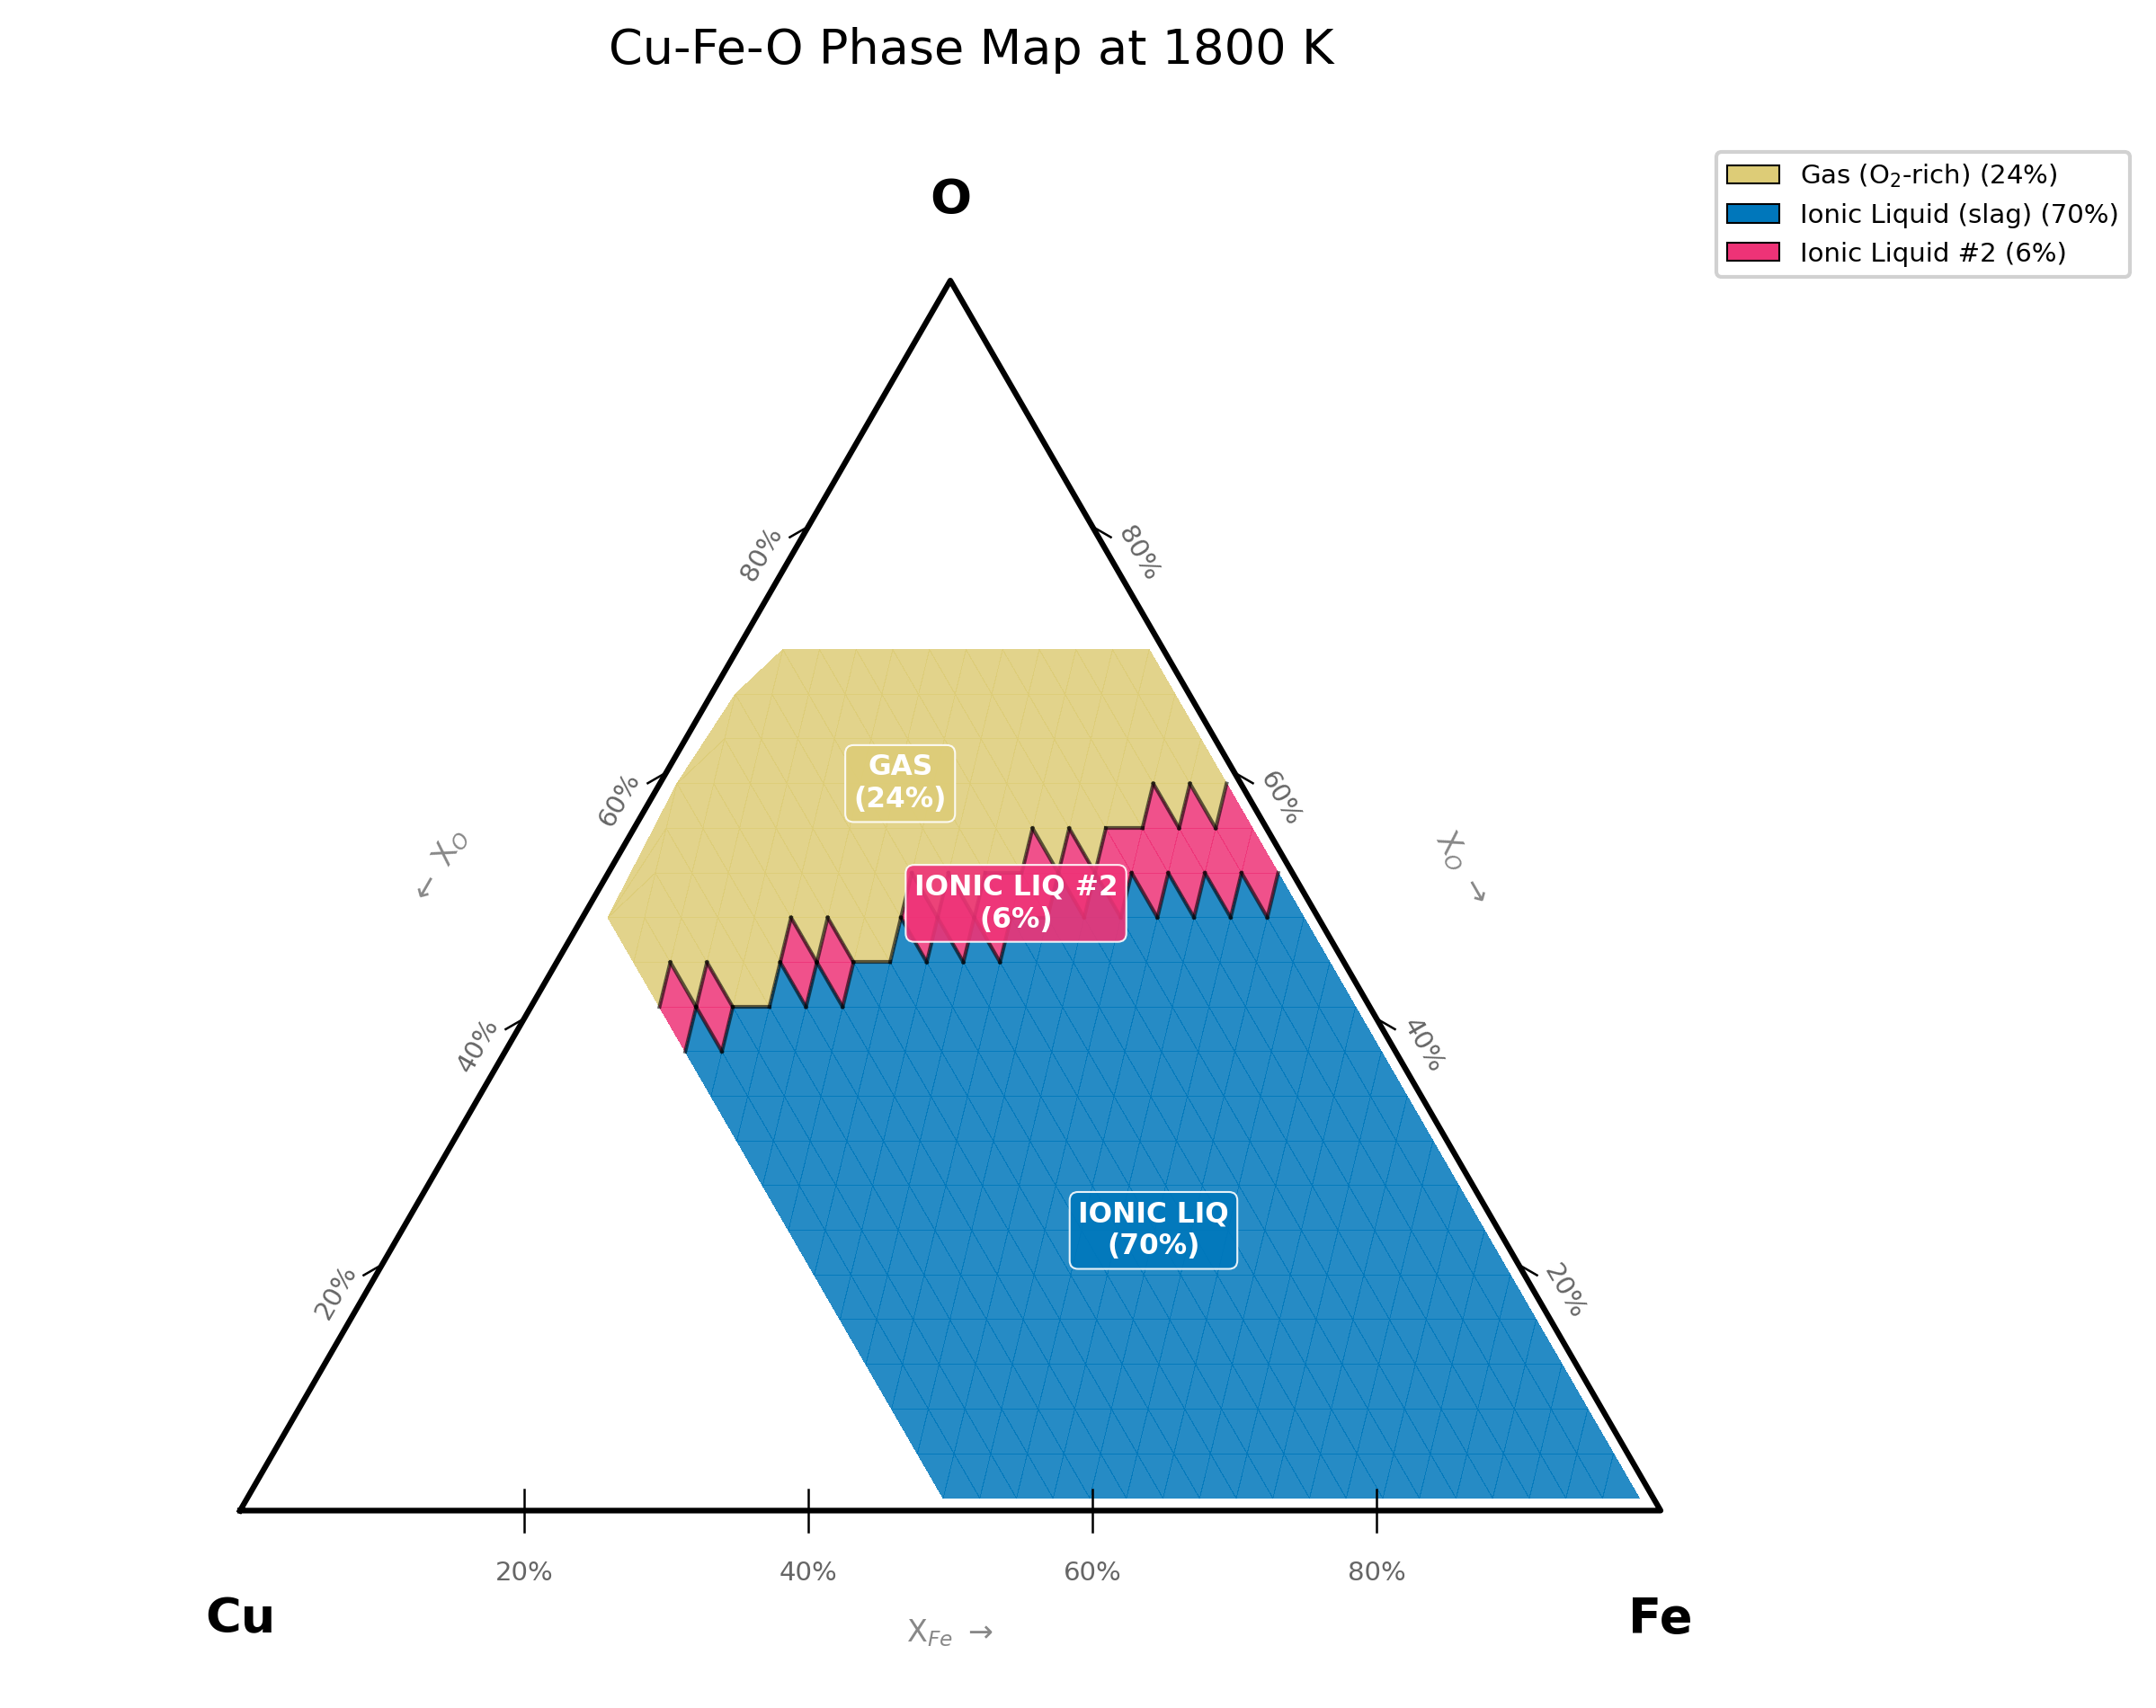
\includegraphics[width=0.8\textwidth]{phase_map_cu_fe_o_1800K.png}
    \caption{Cu-Fe-O phase map at \SI{1800}{\kelvin}. The system is 70\% ionic liquid slag (blue), indicating FeO-based compositions are predominantly molten at steelmaking temperature. The O-rich corner is gas phase (yellow). A narrow immiscible second liquid (magenta, 6\%) appears at the Fe-O boundary, indicating liquid-liquid phase separation.}
    \label{fig:phase_fe}
\end{figure}

\begin{figure}[H]
    \centering
    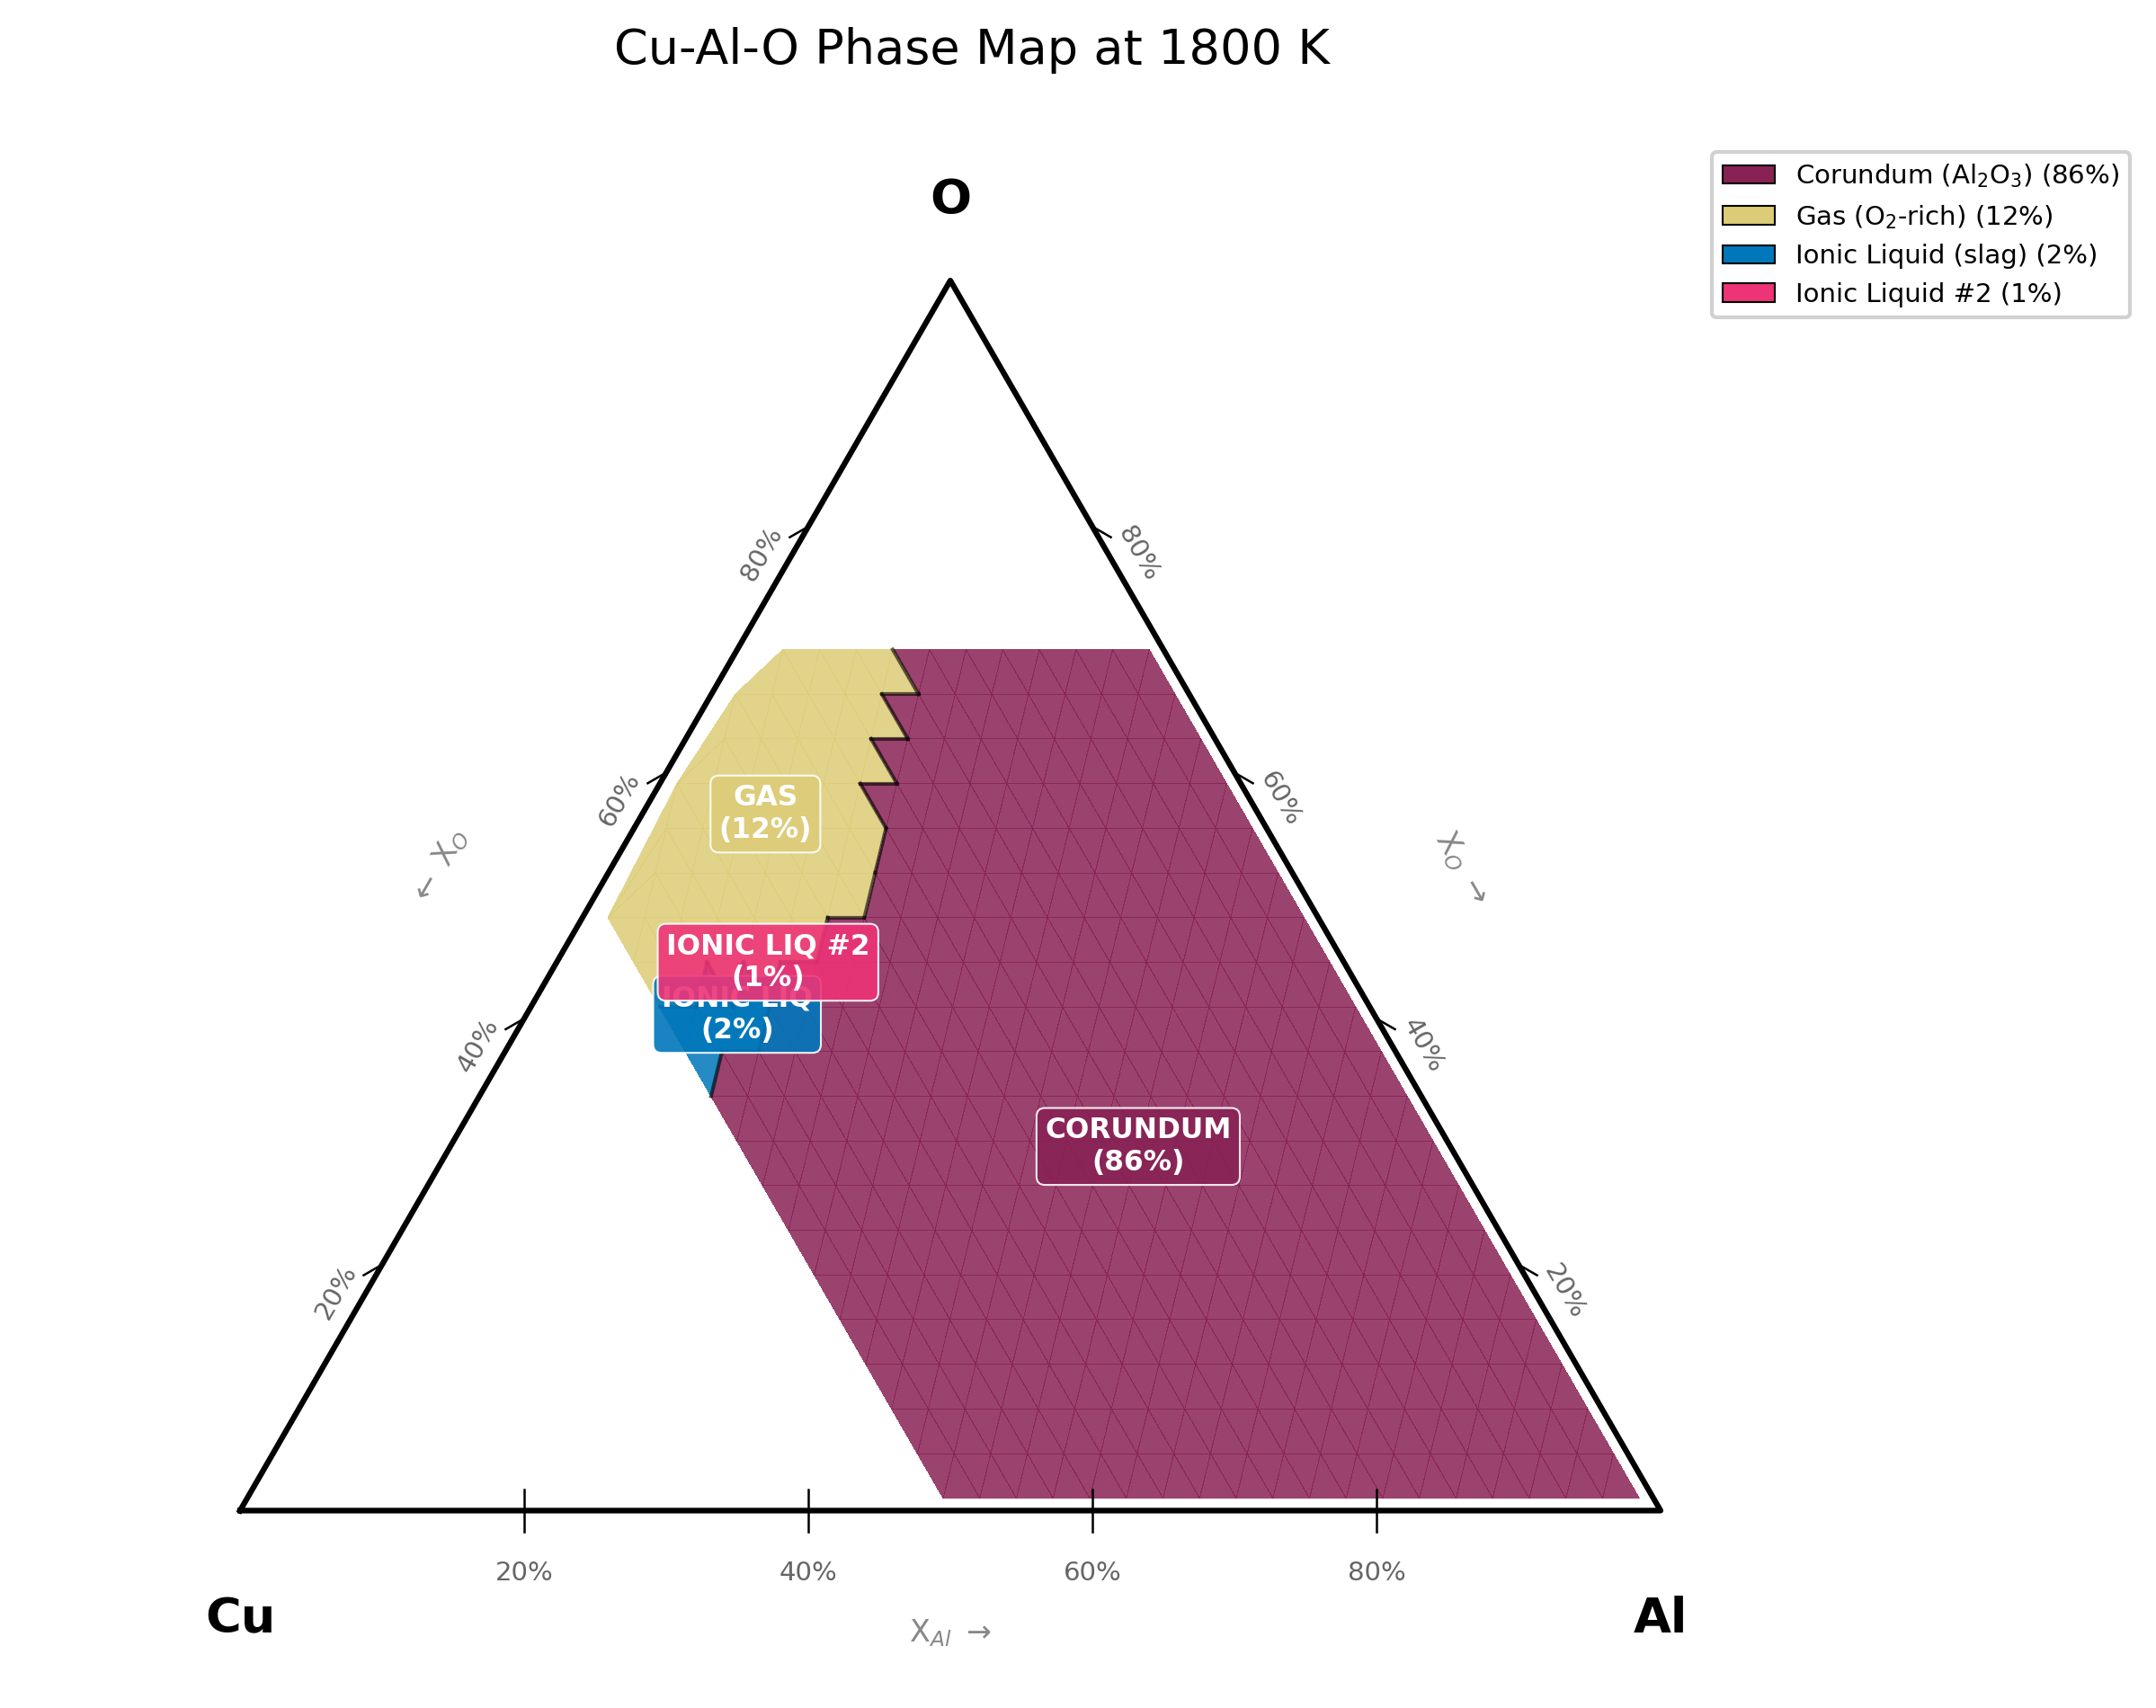
\includegraphics[width=0.8\textwidth]{phase_map_cu_al_o_1800K.png}
    \caption{Cu-Al-O phase map at \SI{1800}{\kelvin}. Dominated by solid corundum (Al$_2$O$_3$, dark wine, 86\%). The limited ionic liquid region (blue, 2\%) confirms that Al$_2$O$_3$ remains solid at steelmaking temperature, restricting Cu capture to solid-liquid interface reactions.}
    \label{fig:phase_al}
\end{figure}

\begin{figure}[H]
    \centering
    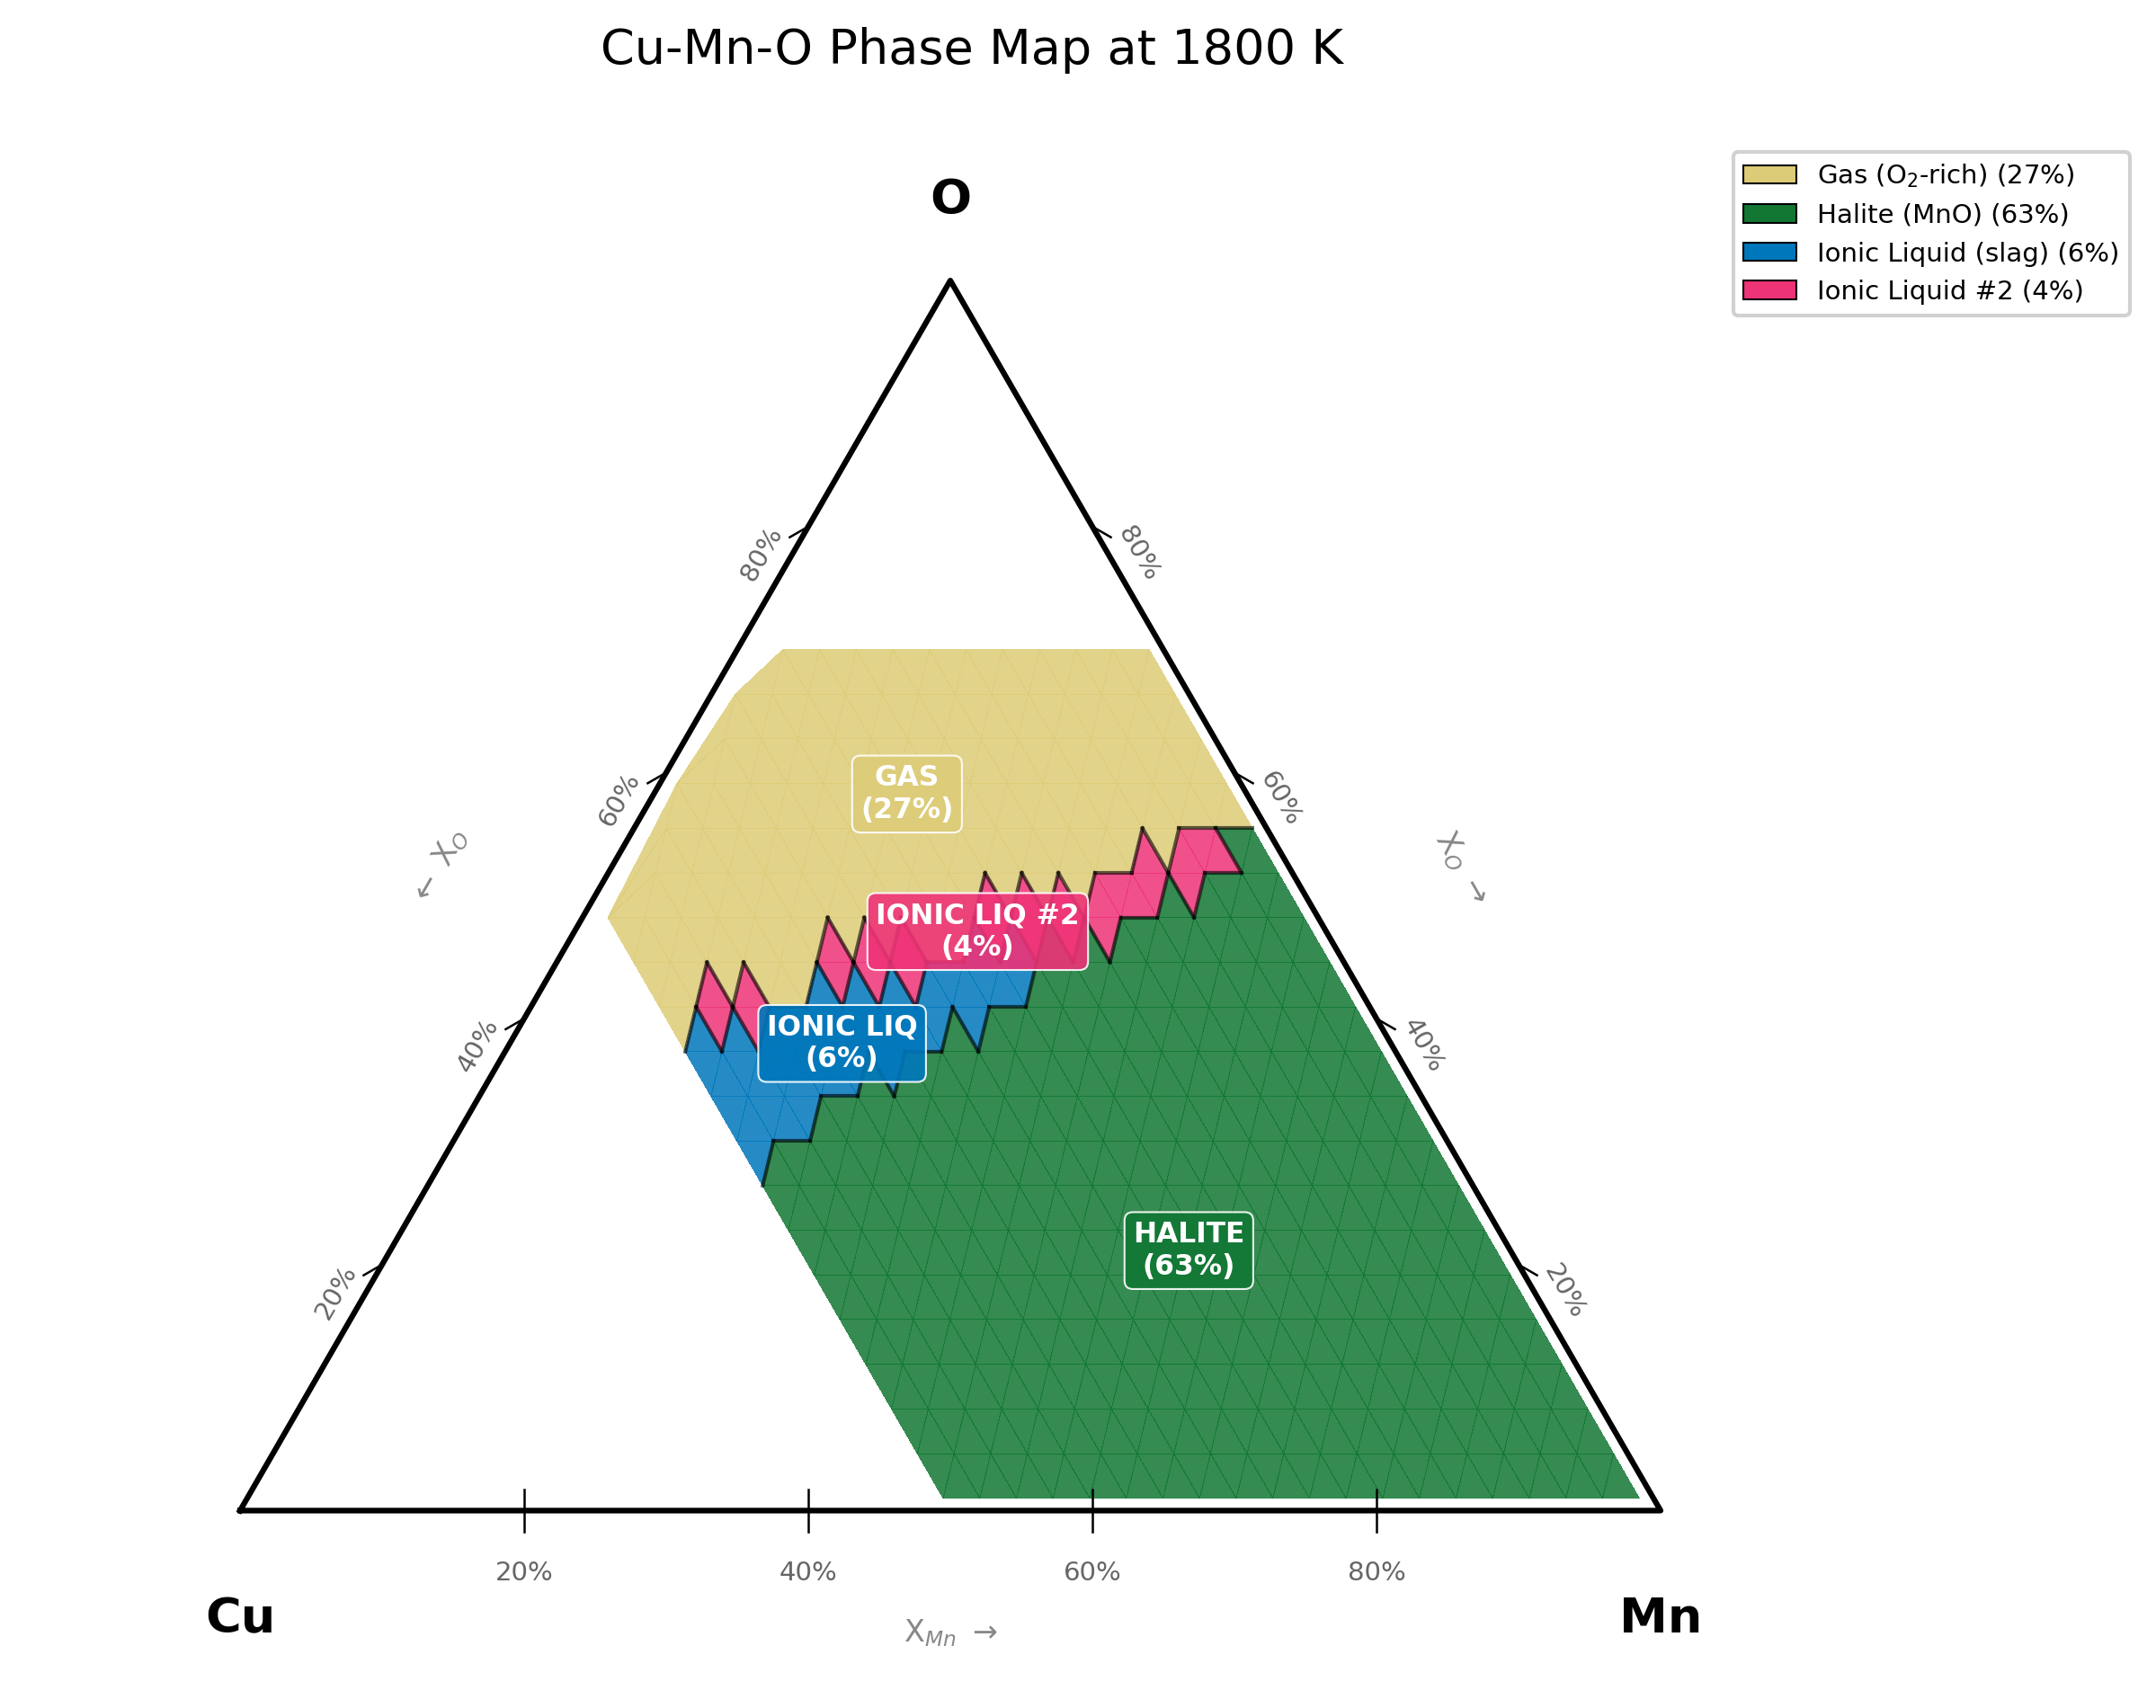
\includegraphics[width=0.8\textwidth]{phase_map_cu_mn_o_1800K.png}
    \caption{Cu-Mn-O phase map at \SI{1800}{\kelvin}. The halite structure (MnO, green, 63\%) dominates the Mn-rich region, with gas (yellow, 27\%) at O-rich compositions. Two immiscible ionic liquids (blue 6\%, magenta 4\%) appear at the Cu-rich boundary, suggesting partial melting occurs even in MnO-dominated systems.}
    \label{fig:phase_mn}
\end{figure}

\subsection{Interpretation}

\begin{table}[H]
\caption{Phase Distribution Summary at \SI{1800}{\kelvin}}
\label{tab:phases}
\centering
\renewcommand{\arraystretch}{1.3}
\setlength{\arrayrulewidth}{0.8pt}
\begin{tabular}{|>{\raggedright\arraybackslash}p{1.2in}|>{\raggedright\arraybackslash}p{2.0in}|>{\centering\arraybackslash}p{0.8in}|>{\raggedright\arraybackslash}p{1.8in}|}
\hline
\rowcolor{headercolor}
\textcolor{white}{\textbf{System}} & \textcolor{white}{\textbf{Dominant Phase}} & \textcolor{white}{\textbf{Fraction}} & \textcolor{white}{\textbf{Implication}} \\
\hline
Cu-Fe-O & IONIC\_LIQ (slag) & 70\% & Fully liquid; good contact with melt \\
\hline
\rowcolor{altrow}
Cu-Al-O & CORUNDUM (solid) & 86\% & Mostly solid; surface reaction only \\
\hline
Cu-Mn-O & HALITE (solid) & 63\% & Mixed; partial melting \\
\hline
\end{tabular}
\end{table}

The Cu-Fe-O system is predominantly liquid at \SI{1800}{\kelvin}, meaning FeO-based slag would have excellent contact with molten steel. This is practically advantageous: liquid slag can coat and permeate through porous filter media, maximizing the reaction surface area for Cu capture.

In contrast, the Cu-Al-O system is 86\% solid corundum. While the $\Delta G$ for CuAl$_2$O$_4$ formation is favorable ($-32$~kJ), the reaction is limited to the solid-liquid interface. This is consistent with Zhang's observation that Al$_2$O$_3$ showed ``some'' Cu reduction in prior experiments but was not as effective as expected.

\textbf{Key insight:} No named ternary crystalline phase (spinel, delafossite, etc.) exists at \SI{1800}{\kelvin} in any system. At steelmaking temperatures, ``Cu capture'' means Cu dissolution into an oxide slag, not crystalline compound formation. The ternary phases (CuFe$_2$O$_4$ spinel, etc.) exist only below $\sim$\SI{1700}{\kelvin}.

%%%%%%%%%%%%%%%%%%%%%%%%%%%%%%%%%%%%%%%%%%%%%%%%%%%%%%%%%%%%%%%%%%%%%%%%%%%%%%%
% 6. SLAG BASICITY EFFECTS
%%%%%%%%%%%%%%%%%%%%%%%%%%%%%%%%%%%%%%%%%%%%%%%%%%%%%%%%%%%%%%%%%%%%%%%%%%%%%%%
\section{Slag Basicity Effects}

\subsection{Method}

Two quaternary systems were investigated at $T = \SI{1800}{\kelvin}$ with $X_{\text{Cu}} = 0.003$ (steelmaking level, $\sim$0.3\%):

\begin{itemize}[leftmargin=*]
    \item \textbf{Cu-Mn-Si-O:} Varied MnO:SiO$_2$ ratio from 0.2 to 3.0
    \item \textbf{Cu-Al-Si-O:} Varied Al$_2$O$_3$:SiO$_2$ ratio from 0.2 to 3.0
\end{itemize}

The basicity ratio (basic oxide : SiO$_2$) controls slag chemistry. A decreasing $a_{\text{Cu}}$ with increasing basicity means the slag is more effective at capturing Cu.

\begin{figure}[H]
    \centering
    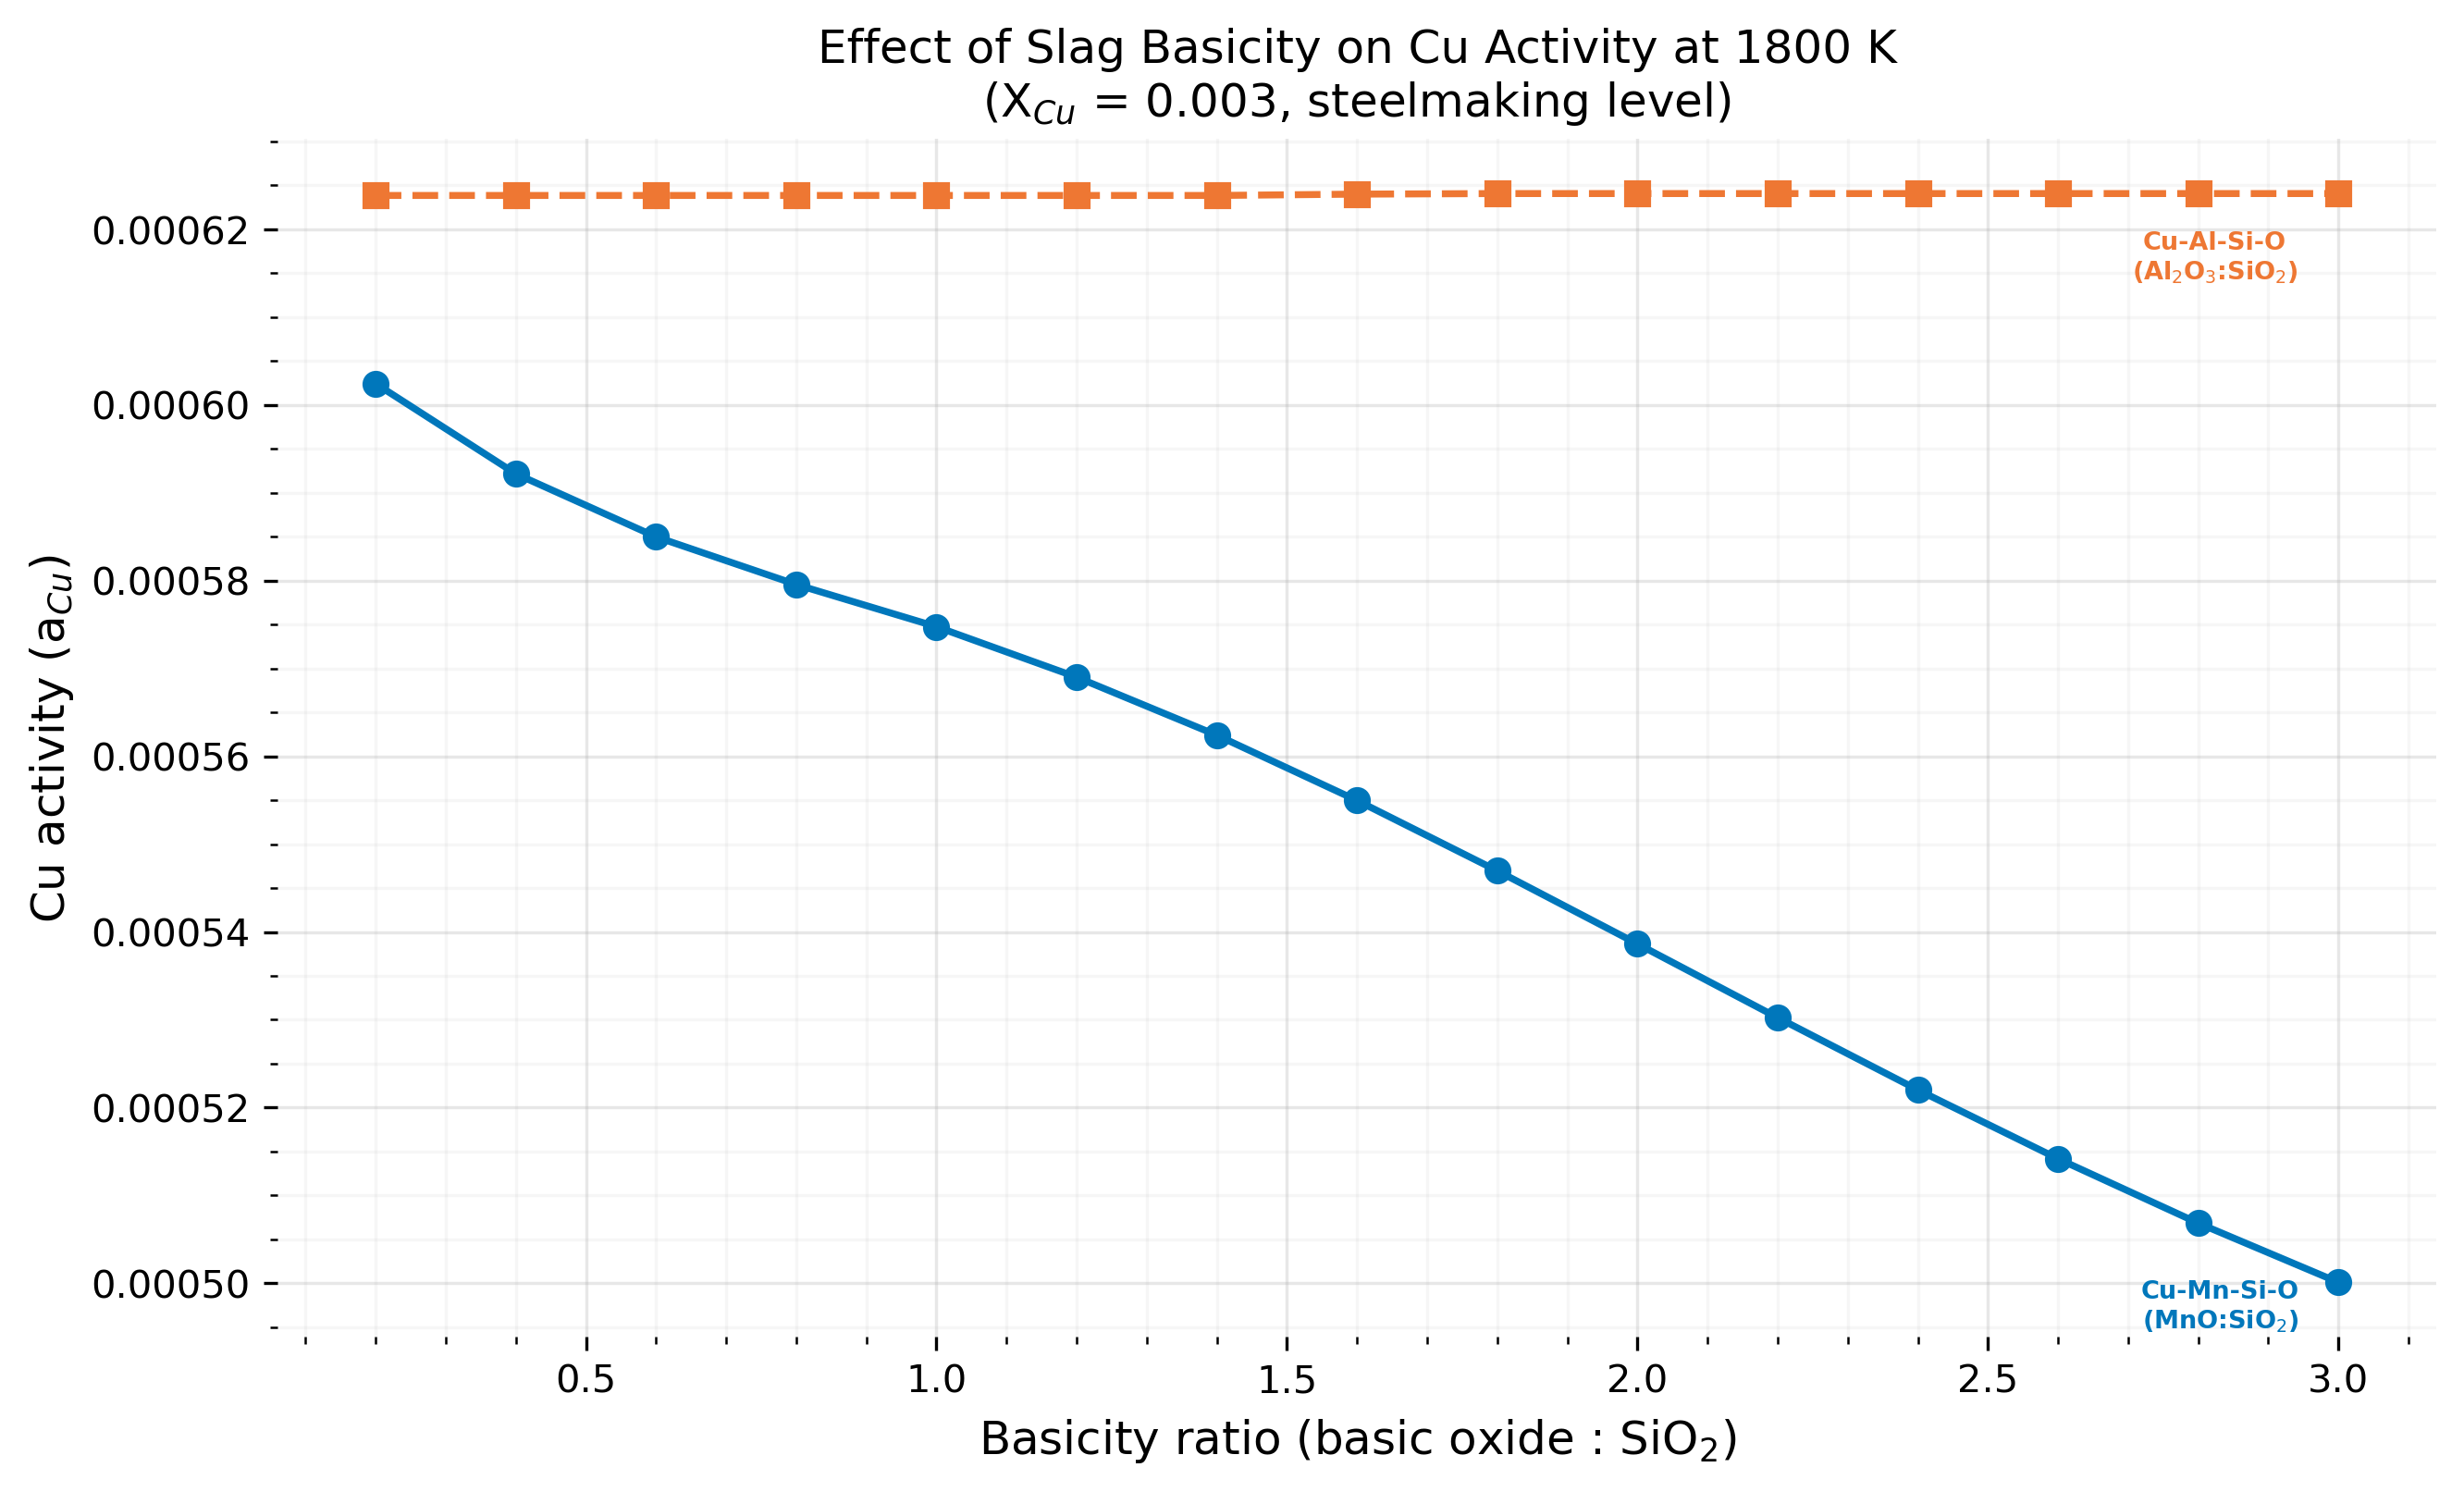
\includegraphics[width=\textwidth]{slag_basicity_vs_aCu.png}
    \caption{Cu activity vs.\ slag basicity ratio at \SI{1800}{\kelvin} with $X_{\text{Cu}} = 0.003$. MnO-SiO$_2$ slag shows a 17\% decrease in $a_{\text{Cu}}$ with increasing basicity, while Al$_2$O$_3$-SiO$_2$ slag is insensitive to basicity.}
    \label{fig:slag}
\end{figure}

\subsection{Results}

\begin{table}[H]
\caption{Slag Basicity Effect on Cu Activity}
\label{tab:slag}
\centering
\renewcommand{\arraystretch}{1.3}
\setlength{\arrayrulewidth}{0.8pt}
\begin{tabular}{|>{\raggedright\arraybackslash}p{1.5in}|>{\centering\arraybackslash}p{1.2in}|>{\centering\arraybackslash}p{1.2in}|>{\centering\arraybackslash}p{1.0in}|}
\hline
\rowcolor{headercolor}
\textcolor{white}{\textbf{System}} & \textcolor{white}{\textbf{$a_{\text{Cu}}$ (low $R$)}} & \textcolor{white}{\textbf{$a_{\text{Cu}}$ (high $R$)}} & \textcolor{white}{\textbf{Trend}} \\
\hline
Cu-Mn-Si-O & 0.000602 & 0.000500 & Decreasing \\
\hline
\rowcolor{altrow}
Cu-Al-Si-O & 0.000572 & 0.000570 & Flat \\
\hline
\end{tabular}
\end{table}

\subsection{Interpretation}

The MnO:SiO$_2$ result is encouraging: higher basicity (more MnO relative to SiO$_2$) drives $a_{\text{Cu}}$ down by $\sim$17\%. In practice, this means slag composition is a tunable lever for optimizing Cu capture. Basic MnO-SiO$_2$ slags would be preferred over neutral compositions.

The insensitivity of the Al$_2$O$_3$-SiO$_2$ system suggests that for alumina-based capture, slag basicity is not a useful optimization parameter. The Cu activity is controlled by other factors (likely the corundum-liquid equilibrium).

%%%%%%%%%%%%%%%%%%%%%%%%%%%%%%%%%%%%%%%%%%%%%%%%%%%%%%%%%%%%%%%%%%%%%%%%%%%%%%%
% 7. Cu ACTIVITY ANALYSIS
%%%%%%%%%%%%%%%%%%%%%%%%%%%%%%%%%%%%%%%%%%%%%%%%%%%%%%%%%%%%%%%%%%%%%%%%%%%%%%%
\section{Cu Activity vs.\ Oxide Fraction}

\subsection{Method}

For four systems (Cu-Al-O, Cu-Mn-O, Cu-Fe-O, Cu-V-O), Cu activity ($a_{\text{Cu}}$) was computed at $T = \SI{1800}{\kelvin}$ while sweeping $X_{\text{Cu}}$ from 0.90 to 0.05 in 20 steps. The non-Cu fraction maintains the oxide stoichiometry (e.g., Al$_2$O$_3$: $X_{\text{Al}}$:$X_{\text{O}}$ = 2:3).

\begin{figure}[H]
    \centering
    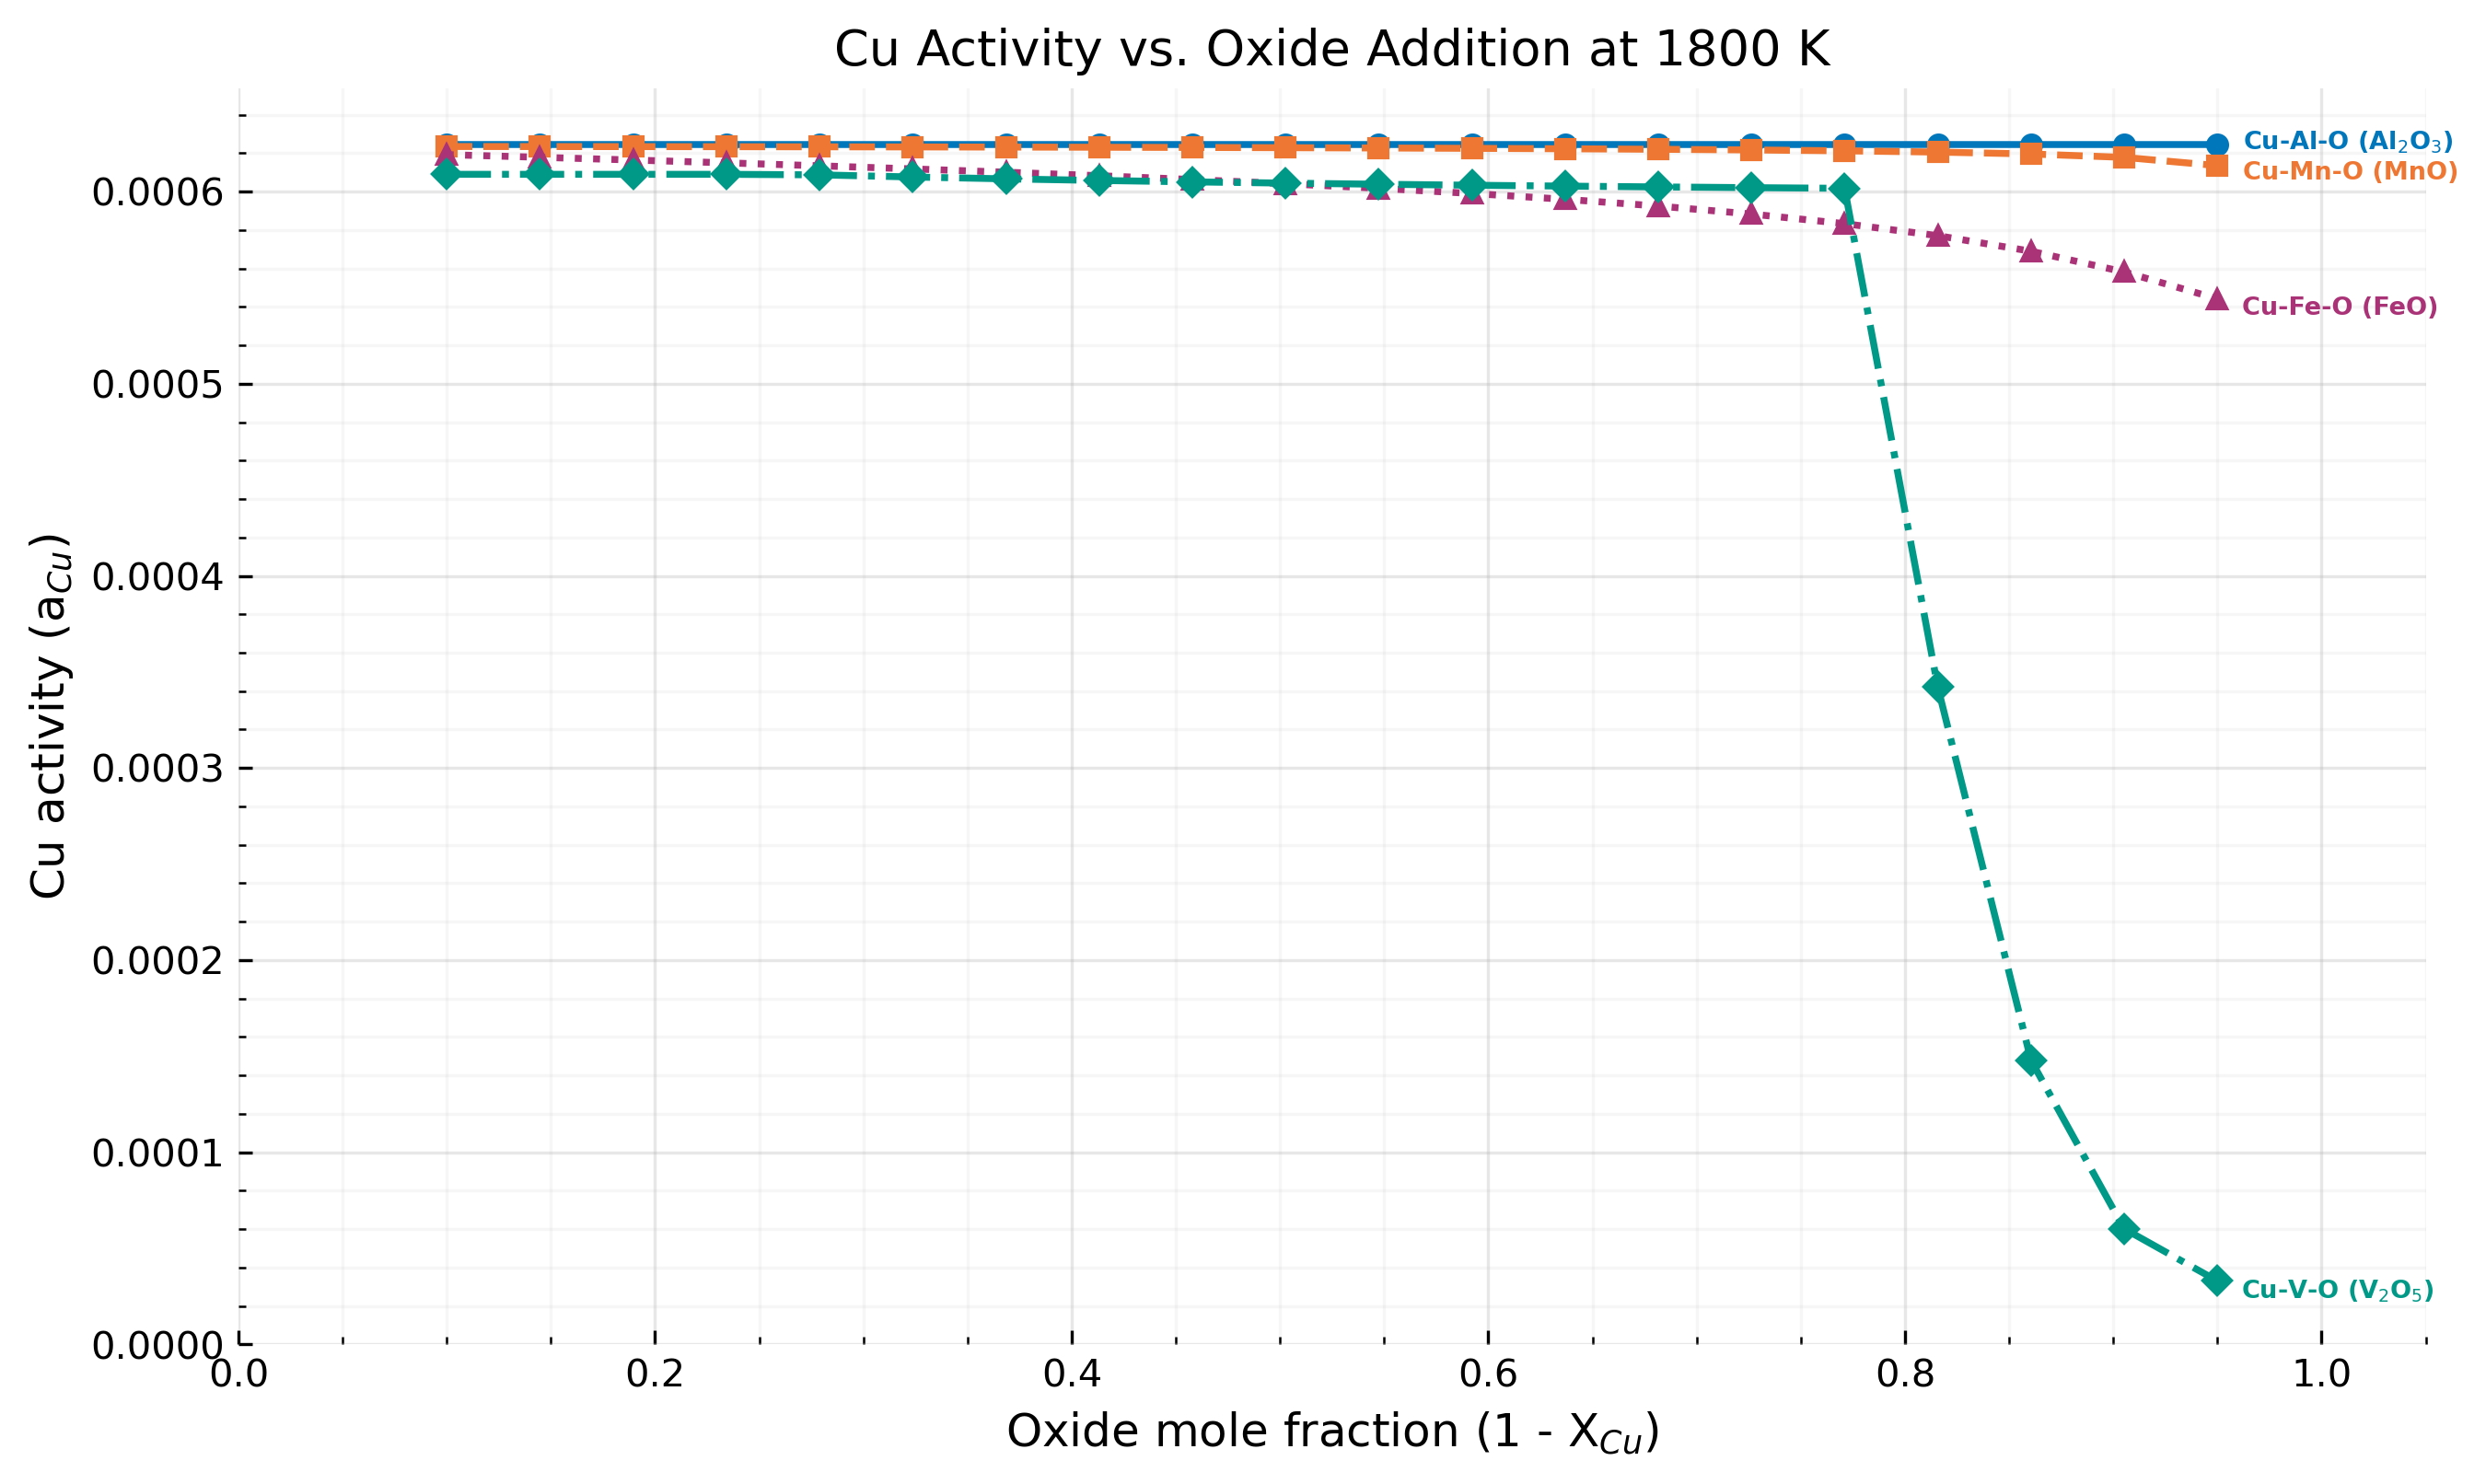
\includegraphics[width=\textwidth]{cu_activity_vs_oxide.png}
    \caption{Cu activity vs.\ oxide mole fraction at \SI{1800}{\kelvin}. All four systems show flat $a_{\text{Cu}}$ across the composition range, a consequence of Gibbs Phase Rule invariance in two-phase fields.}
    \label{fig:activity}
\end{figure}

\subsection{Gibbs Phase Rule Analysis}

The flat $a_{\text{Cu}}$ curves are \textit{not} a computational error. They are a direct consequence of the Gibbs Phase Rule:
\begin{equation}
    F = C - P + 2
\end{equation}

At fixed $T$ and $P$ ($F_{\text{used}} = 2$), a ternary system ($C = 3$) in a two-phase field ($P = 2$) has:
\begin{equation}
    F = 3 - 2 + 2 - 2 = 1
\end{equation}

This single remaining degree of freedom is consumed by the overall composition, but the \textit{compositions} of the two coexisting phases are fixed. Since activity depends on phase composition (not overall composition), $a_{\text{Cu}}$ is invariant across the two-phase field.

\subsection{Physical Meaning}

In the TCOX14 database, there is no separate metallic Cu phase (no FCC\_A1 or LIQUID). All copper dissolves into the ionic liquid (IONIC\_LIQ, a two-sublattice model). The measured $a_{\text{Cu}} \approx 0.0006$ is the real thermodynamic Cu activity set by the Cu-O redox equilibrium at \SI{1800}{\kelvin}.

While this answers a different question than originally intended (we wanted to see $a_{\text{Cu}}$ in metallic Cu drop as oxide is added), the result is still valuable: it confirms that Cu is strongly stabilized in the oxide slag phase (very low activity = strong chemical affinity).

%%%%%%%%%%%%%%%%%%%%%%%%%%%%%%%%%%%%%%%%%%%%%%%%%%%%%%%%%%%%%%%%%%%%%%%%%%%%%%%
% 8. LITERATURE CROSS-CHECK
%%%%%%%%%%%%%%%%%%%%%%%%%%%%%%%%%%%%%%%%%%%%%%%%%%%%%%%%%%%%%%%%%%%%%%%%%%%%%%%
\section{Literature Cross-Check of Computed Values}

To strengthen confidence in our CALPHAD predictions, we surveyed published experimental data for the key Cu-spinel systems. The results confirm that our computed $\Delta G$ values are consistent with independent calorimetric and electrochemical measurements.

\subsection{Key References}

\begin{table}[H]
\caption{Experimental Validation Sources for Top Candidates}
\label{tab:litcheck}
\centering
\renewcommand{\arraystretch}{1.3}
\setlength{\arrayrulewidth}{0.8pt}
\small
\begin{tabular}{|>{\raggedright\arraybackslash}p{1.0in}|>{\raggedright\arraybackslash}p{1.8in}|>{\raggedright\arraybackslash}p{3.0in}|}
\hline
\rowcolor{headercolor}
\textcolor{white}{\textbf{Phase}} & \textcolor{white}{\textbf{Reference}} & \textcolor{white}{\textbf{Key Result}} \\
\hline
CuFe$_2$O$_4$ & Shishin et al.\ (2013), \textit{CALPHAD} 41, 160--179 & Complete CALPHAD assessment of Cu-Fe-O. Spinel modeled with Compound Energy Formalism (9 parameters). Gibbs energy expressions for CuFe$_2$O$_4$ end-member reproduce all available phase equilibria. \\
\hline
\rowcolor{altrow}
CuFe$_2$O$_4$ & Sahu \& Navrotsky (2017), \textit{J.\ Am.\ Ceram.\ Soc.}\ 100, 3684 & High-$T$ oxide melt calorimetry on Fe$_3$O$_4$--CuFe$_2$O$_4$ solid solutions. Negative mixing enthalpy confirmed. \\
\hline
CuAl$_2$O$_4$ & Jacob \& Alcock (1975), \textit{J.\ Am.\ Ceram.\ Soc.}\ 58, 192 & EMF-measured $\Delta G_f$ from 700--1100$^\circ$C using ZrO$_2$ galvanic cells. Directly comparable to our computed $-32$~kJ at 1527$^\circ$C (requires extrapolation above 1100$^\circ$C). \\
\hline
\rowcolor{altrow}
CuAl$_2$O$_4$ & Navrotsky \& Kleppa (1968), \textit{J.\ Inorg.\ Nucl.\ Chem.}\ 30, 479 & $\Delta H_f$(from oxides) $= +21.63 \pm 0.79$~kJ/mol at 970~K. \textbf{Endothermic} from oxides, confirming that the negative $\Delta G$ at high $T$ is entropy-driven ($T\Delta S$ term). \\
\hline
CuMn$_2$O$_4$ & Sahu \& Navrotsky (2017) & Mn$_3$O$_4$--CuMn$_2$O$_4$ shows \textbf{ideal mixing} (zero $\Delta H_{\text{mix}}$). Formation enthalpies from oxides and elements determined. \\
\hline
\rowcolor{altrow}
Cu$_3$V$_2$O$_8$ & Bureau of Mines (via 911Metallurgist summary) & V$_2$O$_5$ was more effective than Al$_2$O$_3$ and MnO$_2$ in oxide injection tests, but results remained far below viable levels. Consistent with our large negative $\Delta G = -109$~kJ at pure-component conditions. \\
\hline
\end{tabular}
\end{table}

\subsection{Physical Consistency Check}

The Navrotsky \& Kleppa (1968) calorimetry data for CuAl$_2$O$_4$ provides a particularly informative cross-check. The \textit{positive} enthalpy of formation from oxides ($+21.63$~kJ/mol) means that at low temperatures, CuAl$_2$O$_4$ formation is endothermic and thermodynamically unfavorable. Our CALPHAD model correctly predicts this: at 800~K, the $\Delta G$ for the full reaction (Cu + Al$_2$O$_3$ + $\frac{1}{2}$O$_2$ $\rightarrow$ CuAl$_2$O$_4$) is only $-62$~kJ, and the compound component is much weaker. At 1800~K, the entropy term ($-T\Delta S$) dominates, making the reaction favorable ($\Delta G = -32$~kJ). This temperature-dependent crossover from enthalpy-controlled to entropy-controlled behavior is exactly what the experimental data predicts.

\subsection{Experimental Decopperization Context}

Recent experimental studies provide context for achievable Cu removal efficiencies:

\begin{itemize}[leftmargin=*]
    \item \textbf{ZnAl$_2$O$_4$ spinel} (2021): Blowing fine-grain powder into steel at 1600$^\circ$C achieved up to \textbf{70\% decopperization}. However, ZnAl$_2$O$_4$ as a filter substrate was ineffective --- Cu infiltrated but did not form stable compounds in the reaction layer.

    \item \textbf{FeO-SiO$_2$-CaCl$_2$ flux} (Shimpo et al., 2013): At 1600$^\circ$C, Cu decreased from 1.87 to 1.11~wt\% (\textbf{$\sim$41\% removal}) via oxidation to Cu$_2$O followed by CaCl$_2$ chlorination.

    \item \textbf{Na$_2$CO$_3$-FeS flux} (Nagasaka et al., 2015): Cu distribution ratio $L_{\text{Cu}} = 24$ at $X_{\text{NaS}_{0.5}} = 0.4$. Sulfide-based fluxes exploit Cu-S affinity rather than oxide formation.

    \item \textbf{Oxysulfide electrorefining} (2024): Cu decreased from 0.43 to below 0.08~wt\% (\textbf{$\sim$81\% removal}) using steelmaking slag-based electrolyte. Non-oxide approach.
\end{itemize}

The ZnAl$_2$O$_4$ result is particularly relevant: it demonstrates that spinel-based Cu capture \textit{can work} experimentally at steelmaking temperatures when the oxide is injected as fine particles, supporting our thermodynamic prediction that CuFe$_2$O$_4$ and CuMn$_2$O$_4$ spinel-forming oxides should be effective.

\subsection{DICTRA / Kinetics Assessment}

A literature survey initially concluded that no oxide mobility database existed. However, VM probing (March 13) revealed:

\begin{itemize}[leftmargin=*]
    \item \textbf{MOBOX1 and MOBOX2 are installed} on the OSU VM, contrary to initial literature findings. These are oxide-phase mobility databases that could potentially enable DICTRA diffusion modeling within slag/spinel phases.

    \item \textbf{MOBFE5--9 are installed} (steel mobility), covering Cu diffusion in metallic Fe-based phases. However, the DICTRA API (\texttt{select\_thermodynamic\_and\_kinetic\_databases\_with\_elements}) could not locate MOBFE9 via the kinetic database discovery method, despite its presence as a standalone database.

    \item \textbf{TCFE+TCOX combined loading fails} due to incompatible CORUNDUM phase descriptions (see Limitation~5). This prevents modeling the full steel-slag interface even if DICTRA could connect.

    \item \textbf{No Process Metallurgy Module} is available on the OSU VM.

    \item \textbf{Unexplored path:} Loading MOBOX directly with TCOX (without TCFE) may enable oxide-phase diffusion modeling. This has not yet been tested.
\end{itemize}

%%%%%%%%%%%%%%%%%%%%%%%%%%%%%%%%%%%%%%%%%%%%%%%%%%%%%%%%%%%%%%%%%%%%%%%%%%%%%%%
% 9. CONCLUSIONS AND NEXT STEPS
%%%%%%%%%%%%%%%%%%%%%%%%%%%%%%%%%%%%%%%%%%%%%%%%%%%%%%%%%%%%%%%%%%%%%%%%%%%%%%%
\section{Conclusions and Next Steps}

\subsection{Activity-Corrected $\Delta G$ Under Steelmaking Conditions}

The pure-component $\Delta G$ values overstate the driving force because Cu is dilute in steel. Under steelmaking conditions ($X_{\text{Cu}} = 0.003$, $\gamma_{\text{Cu}} = 8.5$, $a_{\text{Cu}} = 0.0255$), each Cu atom consumed adds $+RT\ln(1/a_{\text{Cu}}) = +54.9$~kJ at \SI{1800}{\kelvin} to the reaction free energy. Reactions consuming multiple Cu atoms per formula unit are penalized most heavily.

\begin{figure}[H]
    \centering
    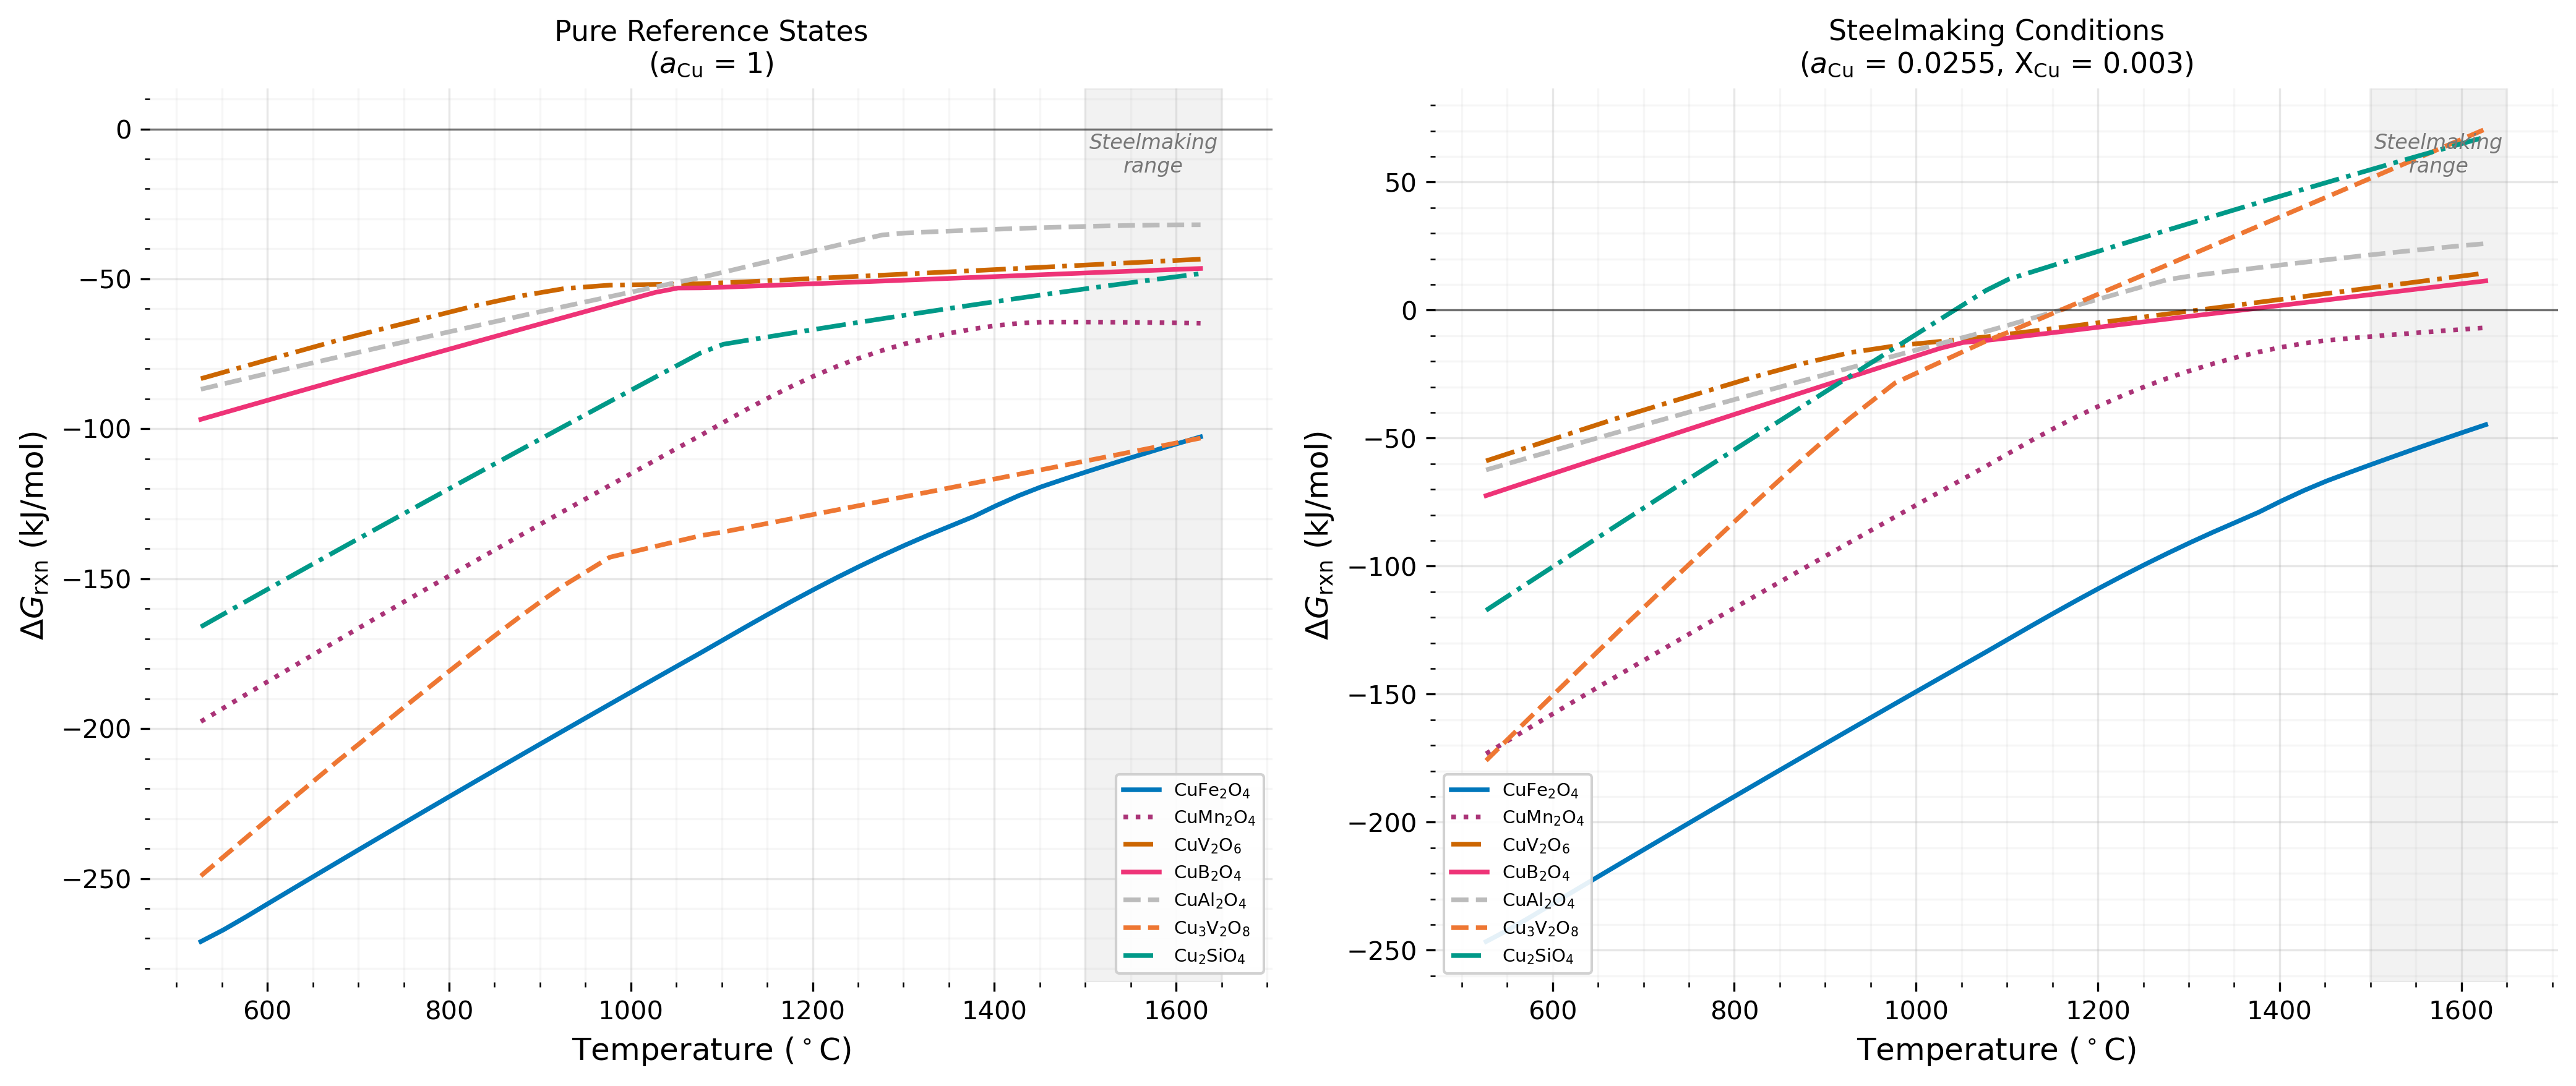
\includegraphics[width=\textwidth]{dG_corrected_comparison.png}
    \caption{Comparison of $\Delta G_{\text{rxn}}$ under pure reference states (left) vs.\ steelmaking conditions (right, $a_{\text{Cu}} = 0.0255$). Only CuFe$_2$O$_4$ and CuMn$_2$O$_4$ remain below zero at steelmaking temperatures. Cu$_3$V$_2$O$_8$ crosses zero because its 3-Cu stoichiometry incurs a $3\times$ activity penalty.}
    \label{fig:dG_corrected}
\end{figure}

\begin{table}[H]
\caption{Activity-Corrected $\Delta G$ at \SI{1800}{\kelvin} ($a_{\text{Cu}} = 0.0255$)}
\label{tab:corrected}
\centering
\renewcommand{\arraystretch}{1.3}
\setlength{\arrayrulewidth}{0.8pt}
\begin{tabular}{|>{\centering\arraybackslash}p{0.3in}|>{\raggedright\arraybackslash}p{1.3in}|>{\centering\arraybackslash}p{0.5in}|>{\centering\arraybackslash}p{0.8in}|>{\centering\arraybackslash}p{0.8in}|>{\centering\arraybackslash}p{1.0in}|>{\centering\arraybackslash}p{0.8in}|}
\hline
\rowcolor{headercolor}
\textcolor{white}{\textbf{\#}} & \textcolor{white}{\textbf{Product}} & \textcolor{white}{\textbf{$n_{\text{Cu}}$}} & \textcolor{white}{\textbf{$\Delta G^\circ$ (kJ)}} & \textcolor{white}{\textbf{Corr. (kJ)}} & \textcolor{white}{\textbf{$\Delta G_{\text{eff}}$ (kJ)}} & \textcolor{white}{\textbf{Verdict}} \\
\hline
1 & CuFe$_2$O$_4$ & 1 & $-111.9$ & $+54.9$ & $-57.0$ & Favorable \\
\hline
\rowcolor{altrow}
2 & CuMn$_2$O$_4$ & 1 & $-64.4$ & $+54.9$ & $-9.5$ & Marginal \\
\hline
3 & CuB$_2$O$_4$ & 1 & $-47.7$ & $+54.9$ & $+7.2$ & Unfavorable \\
\hline
\rowcolor{altrow}
4 & CuAl$_2$O$_4$ & 1 & $-32.3$ & $+54.9$ & $+22.6$ & Unfavorable \\
\hline
5 & Cu$_3$V$_2$O$_8$ & 3 & $-109.2$ & $+164.7$ & $+55.6$ & Unfavorable \\
\hline
\rowcolor{altrow}
6 & Cu$_2$SiO$_4$ & 2 & $-52.2$ & $+109.8$ & $+57.6$ & Unfavorable \\
\hline
\end{tabular}
\end{table}

\subsection{Summary of Findings}

\begin{enumerate}[leftmargin=*]
    \item \textbf{FeO is the only robust Cu-capture oxide} under steelmaking conditions ($\Delta G_{\text{eff}} = -57.0$~kJ). Its single-Cu stoichiometry and strong driving force make it resilient to the dilute-Cu activity penalty.

    \item \textbf{MnO is marginally favorable} ($\Delta G_{\text{eff}} = -9.5$~kJ, $\sim$0.6 $kT$ at \SI{1800}{\kelvin}). It remains a candidate because of basicity-tunability and compatibility with slag chemistry, but kinetic barriers may prevent the reaction from proceeding at this weak driving force.

    \item \textbf{V$_2$O$_5$ fails under real conditions} despite appearing second-best in pure-component analysis. Its 3-Cu stoichiometry (Cu$_3$V$_2$O$_8$) incurs a $3\times$ activity penalty. Bureau of Mines oxide injection tests found V$_2$O$_5$ relatively more effective than other oxides but still far below viable levels, consistent with the thermodynamic penalty at dilute Cu.

    \item \textbf{No solid ternary phase survives at \SI{1800}{\kelvin}.} Cu capture at steelmaking temperatures is a slag dissolution process.

    \item \textbf{Slag basicity is a design lever} for MnO-based systems: increasing MnO:SiO$_2$ ratio decreases $a_{\text{Cu}}$ by 17\%.

    \item \textbf{TCFE+TCOX databases are incompatible} on the OSU VM due to conflicting CORUNDUM phase definitions. Modeling Cu partitioning between metallic steel and oxide slag is not currently possible.
\end{enumerate}

\subsection{Recommended Candidates for Experimental Validation}

Based on activity-corrected thermodynamics, practical, and safety considerations:

\begin{table}[H]
\caption{Recommended Candidates for Fontana Lab Experiments}
\label{tab:recommendations}
\centering
\renewcommand{\arraystretch}{1.3}
\setlength{\arrayrulewidth}{0.8pt}
\begin{tabular}{|>{\centering\arraybackslash}p{0.4in}|>{\raggedright\arraybackslash}p{1.3in}|>{\centering\arraybackslash}p{1.0in}|>{\raggedright\arraybackslash}p{2.5in}|}
\hline
\rowcolor{headercolor}
\textcolor{white}{\textbf{Tier}} & \textcolor{white}{\textbf{Oxide}} & \textcolor{white}{\textbf{$\Delta G_{\text{eff}}$ (kJ)}} & \textcolor{white}{\textbf{Rationale}} \\
\hline
1 & FeO & $-57.0$ & Only oxide with strong corrected driving force; liquid at \SI{1800}{\kelvin}; cheap; 41\% of energy is Cu-capture (not just Fe-oxidation) \\
\hline
\rowcolor{altrow}
2 & MnO & $-9.5$ & Marginal but tunable via slag basicity; low cost; non-toxic; compatible with steelmaking slag \\
\hline
3 & Al$_2$O$_3$ & $+22.6$ & Unfavorable under dilute Cu, but tested last year (spinel mechanism); serves as baseline comparison \\
\hline
\end{tabular}
\end{table}

\subsection{Known Limitations}

These limitations should be stated explicitly in the final report and Zhang presentation:

\begin{enumerate}[leftmargin=*]
    \item \textbf{Pure-component reference states --- now corrected.} Our original $\Delta G$ assumed pure Cu as the reactant. Under steelmaking conditions ($X_{\text{Cu}} = 0.003$, $\gamma_{\text{Cu}} \approx 8.5$, $a_{\text{Cu}} = 0.0255$), the correction is $+n_{\text{Cu}} \cdot RT\ln(1/a_{\text{Cu}})$ per reaction. At \SI{1800}{\kelvin} this adds $+54.9$~kJ per Cu atom consumed. \textbf{Only CuFe$_2$O$_4$ ($-57.0$~kJ) and CuMn$_2$O$_4$ ($-9.5$~kJ) remain favorable.} Cu$_3$V$_2$O$_8$ becomes unfavorable ($+55.6$~kJ) because it consumes 3~Cu atoms ($3 \times 54.9 = +164.7$~kJ correction). See Figure~\ref{fig:dG_corrected} and Table~\ref{tab:corrected}.

    \item \textbf{No kinetics.} Thermodynamics predicts whether a reaction \textit{can} occur, not how fast. VM probing confirmed that \textbf{MOBOX1 and MOBOX2 are installed} on the OSU VM (contrary to initial literature survey). However, DICTRA requires compatible thermodynamic + mobility database pairs, and the API could not establish a working TCFE+MOBFE connection. MOBFE9 is installed but not recognized by the diffusion calculation API. Further investigation is needed to determine if MOBOX can be loaded with TCOX for oxide-phase diffusion modeling.

    \item \textbf{Database extrapolation at high temperature.} TCOX14 is assessed primarily from experimental data below $\sim$\SI{1600}{\kelvin}. At steelmaking temperatures (\SIrange{1773}{1923}{\kelvin}), the Gibbs energy models are extrapolated. Cu-containing ternary compounds (CuFe$_2$O$_4$, Cu$_3$V$_2$O$_8$, etc.) have especially sparse high-temperature data. Values at \SIrange{1000}{1400}{\kelvin} are more reliable than those at \SI{1800}{\kelvin}.

    \item \textbf{Missing phases.} TC-Python only finds phases that are assessed in the database. If a Cu-M-O compound exists but was not modeled in TCOX14, it will not appear. The ``always liquid'' result for Cu$_3$V$_2$O$_8$ may mean the solid vanadate phase was never assessed, not that it truly does not exist.

    \item \textbf{TCFE+TCOX databases are incompatible.} Script~2 (Cu activity) could not model Cu partitioning between metallic steel and oxide slag because TCOX14 lacks FCC\_A1 (austenite). VM testing confirmed that loading TCFE13+TCOX14 together fails due to incompatible phase definitions: the CORUNDUM phase has different sublattice models in the two databases (\texttt{INCOMPATIBLE PHASE DESCRIPTION}). All three TCFE versions (13, 12, 11) exhibit this conflict. Modeling the full steel-slag system would require Thermo-Calc to release a unified database or a custom TDB file merging both descriptions.

    \item \textbf{Limited experimental anchors.} Published Cu-removal data includes Bureau of Mines V$_2$O$_5$ injection tests (relatively more effective than Al$_2$O$_3$/MnO$_2$ but far below viable), ZnAl$_2$O$_4$ spinel injection ($\sim$70\% by powder blowing; $\sim$33\% by filter), and FeO-SiO$_2$-CaCl$_2$ flux ($\sim$40\% removal). Calorimetric data exists for CuFe$_2$O$_4$, CuAl$_2$O$_4$, and CuMn$_2$O$_4$ (Navrotsky \& Kleppa 1968; Sahu \& Navrotsky 2017), but most measurements are below 1400~K --- high-temperature validation remains sparse.
\end{enumerate}

\subsection{Paths to Stronger Predictions}

\begin{enumerate}[leftmargin=*]
    \item \textbf{Activity-corrected $\Delta G$ --- COMPLETED.} See Section~\ref{fig:dG_corrected} and Table~\ref{tab:corrected}. The correction ($a_{\text{Cu}} = 0.0255$) eliminates 4 of 6 candidates, leaving only FeO (robust) and MnO (marginal).

    \item \textbf{Kinetic modeling (DICTRA):} MOBOX1 and MOBOX2 are installed on the OSU VM but have not been tested with TCOX. If MOBOX can load alongside TCOX14, oxide-phase diffusion modeling may be possible --- predicting ``how fast'' Cu transfers into slag, not just ``will it.'' The DICTRA API exists but could not connect MOBFE9 via the standard discovery method. Further investigation is needed.

    \item \textbf{Combined TCFE+TCOX database --- BLOCKED.} VM testing confirmed that TCFE (all versions 11--13) and TCOX14 have incompatible CORUNDUM phase definitions. Modeling Cu partitioning between metallic steel and oxide slag would require Thermo-Calc to release a unified database or a custom TDB file merging both phase descriptions.

    \item \textbf{Quantitative literature comparison:} Navrotsky \& Kleppa (1968) and Sahu \& Navrotsky (2017) provide formation enthalpies for CuFe$_2$O$_4$, CuAl$_2$O$_4$, and CuMn$_2$O$_4$. The Shishin et al.\ (2013) CALPHAD assessment of Cu-Fe-O includes optimized Gibbs energy expressions for CuFe$_2$O$_4$ that should be directly compared to our TCOX14 values. Jacob \& Alcock (1975) provide EMF-measured $\Delta G_f$ for CuAl$_2$O$_4$ from 700--1100$^\circ$C. Extracting quantitative values from these papers and overlaying them on our $\Delta G$ vs.\ $T$ curves would strongly validate (or reveal discrepancies in) our TCOX14 predictions.

    \item \textbf{Experimental design informed by models:} Use the phase maps and activity-corrected $\Delta G$ ranking to design experiments that test the key prediction: FeO-based slag should remove more Cu than Al$_2$O$_3$ at \SI{1800}{\kelvin}. Measure Cu concentration in steel before/after oxide contact (via XRF or ICP-OES) and compare the removal efficiency ranking to our computed $\Delta G_{\text{eff}}$ ranking.
\end{enumerate}

\subsection{VM Capabilities Summary (March 13, 2026)}

\begin{enumerate}[leftmargin=*]
    \item \textbf{Thermodynamic databases:} TCOX9--14, TCFE10--13, SSUB3--6, TCAL6--8, TCCU2--4 all installed
    \item \textbf{Mobility databases:} MOBFE5--9, MOBOX1--2, MOBCU1--3, MOBNI3--5, MOBAL1--2 all installed
    \item \textbf{TCFE+TCOX:} INCOMPATIBLE --- CORUNDUM phase conflict in all combinations tested
    \item \textbf{DICTRA API:} Exists but cannot discover MOBFE9 via kinetic database method
    \item \textbf{Process Metallurgy Module:} Not available
    \item \textbf{Untested:} MOBOX+TCOX direct loading for oxide-phase diffusion
\end{enumerate}

%%%%%%%%%%%%%%%%%%%%%%%%%%%%%%%%%%%%%%%%%%%%%%%%%%%%%%%%%%%%%%%%%%%%%%%%%%%%%%%
% APPENDIX
%%%%%%%%%%%%%%%%%%%%%%%%%%%%%%%%%%%%%%%%%%%%%%%%%%%%%%%%%%%%%%%%%%%%%%%%%%%%%%%
\newpage
\appendix
\section{Full Ranking of All 16 Ternary Products}

\begin{table}[H]
\caption{Complete Ternary Product Ranking at \SI{1800}{\kelvin} (\SI{1527}{\celsius})}
\label{tab:full_ranking}
\centering
\renewcommand{\arraystretch}{1.2}
\setlength{\arrayrulewidth}{0.8pt}
\small
\begin{tabular}{|>{\centering\arraybackslash}p{0.3in}|>{\raggedright\arraybackslash}p{1.3in}|>{\centering\arraybackslash}p{0.9in}|>{\raggedright\arraybackslash}p{1.2in}|>{\centering\arraybackslash}p{0.8in}|>{\raggedright\arraybackslash}p{1.0in}|}
\hline
\rowcolor{headercolor}
\textcolor{white}{\textbf{\#}} & \textcolor{white}{\textbf{Product}} & \textcolor{white}{\textbf{$\Delta G$ (kJ)}} & \textcolor{white}{\textbf{Named Phase}} & \textcolor{white}{\textbf{Stable To}} & \textcolor{white}{\textbf{Tier}} \\
\hline
1 & CuFe$_2$O$_4$ & $-111.9$ & SPINEL\#1 & \SI{1700}{\kelvin} & Strong \\
\hline
\rowcolor{altrow}
2 & Cu$_3$V$_2$O$_8$ & $-109.2$ & -- & liquid & Strong \\
\hline
3 & CuMn$_2$O$_4$ & $-64.4$ & SPINEL\#1 & \SI{1700}{\kelvin} & Strong \\
\hline
\rowcolor{altrow}
4 & Cu$_2$SiO$_4$ & $-52.2$ & -- & liquid & Strong \\
\hline
5 & CuB$_2$O$_4$ & $-47.7$ & CUB2O4\#1 & \SI{1300}{\kelvin} & Strong \\
\hline
\rowcolor{altrow}
6 & CuV$_2$O$_6$ & $-45.0$ & -- & liquid & Moderate \\
\hline
7 & CuTiO$_3$ & $-36.8$ & -- & liquid & Moderate \\
\hline
\rowcolor{altrow}
8 & CuCo$_2$O$_4$ & $-35.8$ & SPINEL\#1 & \SI{1150}{\kelvin} & Moderate \\
\hline
9 & CuAl$_2$O$_4$ & $-32.3$ & SPINEL\#1 & \SI{1550}{\kelvin} & Moderate \\
\hline
\rowcolor{altrow}
10 & CuCaO$_2$ & $-30.7$ & -- & -- & Moderate \\
\hline
11 & CuAlO$_2$ & $-30.1$ & DELAFOSSITE & \SI{1550}{\kelvin} & Moderate \\
\hline
\rowcolor{altrow}
12 & CuCr$_2$O$_4$ & $-30.0$ & SPINEL\#1 & \SI{1450}{\kelvin} & Moderate \\
\hline
13 & CuLaO$_2$ & $-27.8$ & DELAFOSSITE & \SI{1500}{\kelvin} & Moderate \\
\hline
\rowcolor{altrow}
14 & CuNiO$_2$ & $-27.3$ & -- & liquid & Moderate \\
\hline
15 & CuSiO$_3$ & $-26.2$ & -- & liquid & Moderate \\
\hline
\rowcolor{altrow}
16 & CuMgO$_2$ & $-26.1$ & -- & -- & Moderate \\
\hline
17 & CuZrO$_3$ & $-25.3$ & -- & liquid & Moderate \\
\hline
\end{tabular}
\end{table}

\section{CuFe$_2$O$_4$ Decomposition Across Temperature}

\begin{table}[H]
\caption{CuFe$_2$O$_4$ Energy Components vs.\ Temperature (Selected Points)}
\label{tab:decomp_full}
\centering
\renewcommand{\arraystretch}{1.2}
\setlength{\arrayrulewidth}{0.8pt}
\small
\begin{tabular}{|>{\centering\arraybackslash}p{0.5in}|>{\centering\arraybackslash}p{0.5in}|>{\centering\arraybackslash}p{1.0in}|>{\centering\arraybackslash}p{1.0in}|>{\centering\arraybackslash}p{1.0in}|>{\centering\arraybackslash}p{0.8in}|}
\hline
\rowcolor{headercolor}
\textcolor{white}{\textbf{$T$ (K)}} & \textcolor{white}{\textbf{$T$ ($^\circ$C)}} & \textcolor{white}{\textbf{Original (kJ)}} & \textcolor{white}{\textbf{Cu-capture (kJ)}} & \textcolor{white}{\textbf{Fe-ox (kJ)}} & \textcolor{white}{\textbf{Cu \%}} \\
\hline
800 & 527 & $-271.0$ & $-85.3$ & $-185.7$ & 31.5 \\
\hline
\rowcolor{altrow}
1000 & 727 & $-235.7$ & $-73.2$ & $-162.4$ & 31.1 \\
\hline
1200 & 927 & $-200.5$ & $-61.2$ & $-139.3$ & 30.5 \\
\hline
\rowcolor{altrow}
1400 & 1127 & $-166.0$ & $-49.8$ & $-116.2$ & 30.0 \\
\hline
1600 & 1327 & $-135.5$ & $-42.5$ & $-93.0$ & 31.3 \\
\hline
\rowcolor{altrow}
1800 & 1527 & $-111.9$ & $-45.7$ & $-66.2$ & 40.8 \\
\hline
1900 & 1627 & $-102.7$ & $-46.7$ & $-56.0$ & 45.5 \\
\hline
\end{tabular}
\end{table}

Note the Cu-capture fraction increases from 31\% at \SI{800}{\kelvin} to 46\% at \SI{1900}{\kelvin}, showing that the copper affinity mechanism becomes relatively more dominant at higher temperatures.

\end{document}
